\documentclass[12pt,a4paper]{report}

\usepackage[utf8]{inputenc}
\usepackage[T1]{fontenc}
\usepackage{combelow}
\usepackage[romanian]{babel}
\usepackage{graphicx}
\usepackage{subfiles}
\usepackage{blindtext}
\usepackage[export]{adjustbox} 
\usepackage{geometry}
\usepackage[nottoc,notlot,notlof]{tocbibind}
\usepackage{indentfirst}
\usepackage{amsthm}
\usepackage{listings}
\usepackage{float}
\usepackage[toc,page]{appendix}
\usepackage{subcaption}
\usepackage{makeidx}
\usepackage{geometry}
\usepackage[verbose]{newunicodechar}
\usepackage{hyperref}
\usepackage{amsmath} 
\usepackage{xparse}
\usepackage[utf8]{inputenc}
\usepackage{chngcntr}
\usepackage{mathtools}
\usepackage[section]{placeins}
\graphicspath{{figures/}}
\usepackage{array}
\usepackage{afterpage}
\usepackage[font=small,labelfont=bf]{caption}

\usepackage{booktabs}
\usepackage{multirow}
\usepackage{color}

\usepackage{listings}
 
\definecolor{codegreen}{rgb}{0,0.6,0}
\definecolor{codegray}{rgb}{0.5,0.5,0.5}
\definecolor{codepurple}{rgb}{0.58,0,0.82}
\definecolor{backcolour}{rgb}{0.95,0.95,0.92}
 
\lstdefinestyle{mystyle}{
    backgroundcolor=\color{backcolour},   
    commentstyle=\color{codegreen},
    keywordstyle=\color{magenta},
    numberstyle=\tiny\color{codegray},
    stringstyle=\color{codepurple},
    basicstyle=\footnotesize,
    breakatwhitespace=false,         
    breaklines=true,                 
    captionpos=b,                    
    keepspaces=true,                 
    numbers=left,                    
    numbersep=5pt,                  
    showspaces=false,                
    showstringspaces=false,
    showtabs=false,                  
    tabsize=2
}
 
\lstset{style=mystyle}

\geometry{
	a4paper,
	total={170mm,257mm},
	left=25mm,
	top=25mm,
	bottom=25mm,
	right=25mm,
}

% Line spacing
\renewcommand{\baselinestretch}{1.5} 
\renewcommand\appendixtocname{Anexe}
\renewcommand\appendixname{Anexe}
\renewcommand\appendixpagename{Anexe}
\newcommand\blankpage{%
	\null
	\thispagestyle{empty}%
	\addtocounter{page}{-1}%
	\newpage}
\newcommand*\xor{\mathbin{\oplus}}
\renewcommand\lstlistlistingname{Listă fragmente de cod}


\DeclarePairedDelimiter\norm{\lVert}{\rVert}%
\DeclarePairedDelimiter\abs{\lvert}{\rvert}%

\graphicspath{{images/}{../images/}{figures/}{../figures/}}

\newunicodechar{ș}{\c{s}}
\newunicodechar{Ș}{\c{S}}
\newunicodechar{ț}{\c{t}}
\newunicodechar{Ț}{\c{T}}

\newtheorem{remark}{Observație}[chapter]
\newtheorem{definition}{Definiție}[chapter]
\newtheorem{lemma}{Lemă}[chapter]
\newtheorem{theorem}{Teoremă}[chapter]

\makeindex

\begin{document}

\afterpage{\blankpage}
\subfile{chapters/0_first_page}
\restoregeometry

\setcounter{page}{3}
\subfile{chapters/01_abstract_ro}

\newpage
\subfile{chapters/01_abstract_en}

\tableofcontents

\newpage
\addcontentsline{toc}{chapter}{\listfigurename}
\listoffigures

\newpage
\addcontentsline{toc}{chapter}{Listă de tabele}
\listoftables

\newpage
\addcontentsline{toc}{chapter}{Listă fragmente de cod}
\lstlistoflistings

\newpage\null\newpage
\chapter{Introducere}
\section{Motivație}

Volumul de date crește semnificativ de la an la an astfel până în 2020 se estimează că pentru fiecare persoană de pe planetă vor fi creați în fiecare secundă 1.7 MB de date, ceea ce înseamnă peste 13 milioane de GB creați în fiecare secundă în lume.

În 2018 în fiecare minut se vizionau peste 97 de mii de ore de conținut pe Netlfix. Peste 4.3 milioane de videoclipuri erau vizionate pe Youtube. Pe Spotify se ascultau 750 de mii de melodii, iar Amazon pregătea peste o mie de pachete.

\section{Obiective propuse}


\section{Actualitate}


\section{Structura lucrării}

\newpage\null\newpage
\chapter{Fundamente teoretice}
\section{Sisteme de recomandare}

\subsection{Noțiuni generale}

Sistemele de recomandare au scopul de oferi sugestii cât mai relevante de articole utilizatorilor unei platforme pe baza unor strategii. Un sistem de recomandare poate folosi una sau mai multe strategii de recomandare după cum vom vedea în continuare. În cazul în care se folosesc cel puțin două strategii, sistemul de recomandare devine un sistem de recomandare hibrid. Prin folosirea mai multor strategii se urmărește ca fiecare strategie să vină în completarea celorlalte strategi cu avantajele sale. De cele mai multe ori, în implementarea unui sistem de recomandare, se folosește tehnica de filtrare coloborativă împreună cu o altă strategie de recomandare \hyperlink{ErionCanoMaurizioMorisio}{[4]}.

\subsection{Strategii de recomandare}

\subsubsection*{Filtrarea coloborativă}

Filtrarea coloborativă se bazează pe faptul că utilizatorii care au în prezent preferințe similare vor avea și în viitor preferințe destul de similare. Această abordare folosește ratingurile pe care le dau utilizatorii sau oricare altă formă de a da un feedback, îmi place/nu îmi place, pentru a identifica preferințele comune dintre grupurile de utilizatori. Odată identificate preferințele se generează recomandări pe baza similarităților dintre utilizatori. 

Dezavantajul acestei strategii apare în momentul în care în sistem intră un nou utilizator. Datorită faptului că utilizatorul este nou, sistemul nu are un istoric al preferințelor lui, iar în consecință nu îl poate asigna unui grup de utilizatori pe baza preferințelor \hyperlink{ErionCanoMaurizioMorisio}{[4]}.
\begin{figure}[!h]
	\centering
	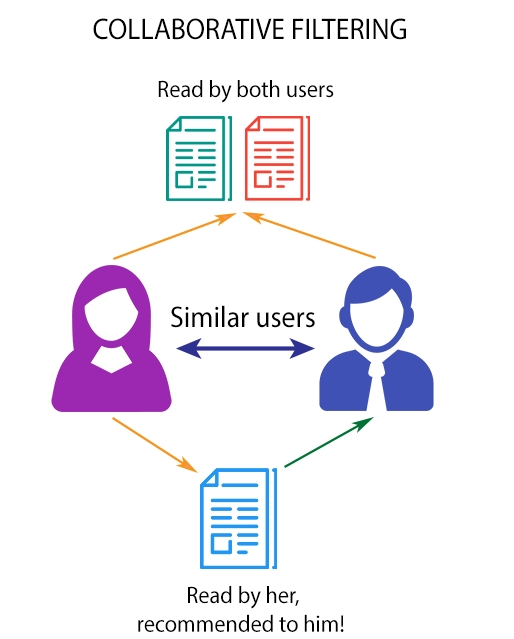
\includegraphics[max width=10cm,max height=10cm,keepaspectratio]{img_2_1}
	\caption[Filtrarea coloborativă]{Filtrarea coloborativă. Imagine preluată din \hyperlink{datameetsmedia}{[5]}.}
\end{figure} 

\subsubsection*{Filtrarea bazată pe conținut}

Filtrarea bazată pe conținut pleacă de la premisa că utiliztorii cărora le-au plăcut articole definite de anumite caracteristici în trecut, vor aprecia aceleași tip de articole și în viitor. Această abordare folosește caracteristicile articolelor pentru a le compara cu profilul utilizatorilor și a oferi recomandări. Calitatea recomandărilor rezultate folosind această strategie este influențată de setul de caracteristici ales pentru articole. Similar cu filtrarea coloborativă, filtrarea bazată pe conținut prezintă dezavantaje în momentul în care în sistem intră un nou utilizator fără istoric \hyperlink{ErionCanoMaurizioMorisio}{[4]}.
\begin{figure}[!h]
	\centering
	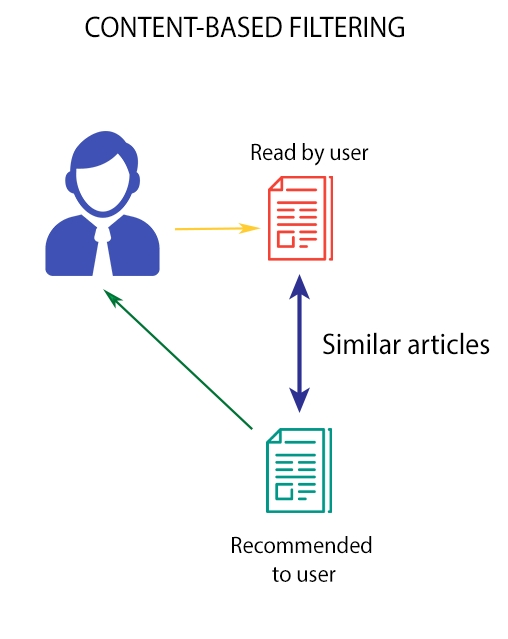
\includegraphics[max width=10cm,max height=10cm,keepaspectratio]{img_2_2}
	\caption[Filtrarea bazată pe conținut]{Filtrarea bazată pe conținut. Imagine preluată din \hyperlink{datameetsmedia}{[5]}.}
\end{figure} 

\subsubsection*{Filtrarea demografică}

Filtrarea demografică folosește atribute precum vârsta, genul, educația, etc. pentru a identifica categoriile de utilizatori. Nu prezintă dezavantaje atunci când apar noi utilizatori în sistem și nu se folosește de ratinguri, sau alt sistem de feedback, pentru a face recomandări.

Dezavantajul este reprezentat de faptul că procesul de colectare al datelor demografice poate fi îngreunat de legislație, fapt ce reprezintă o limitare a acestei metode \hyperlink{ErionCanoMaurizioMorisio}{[4]}.

\subsubsection*{Filtrarea bazată pe cunoștințe}

Filtrarea bazată pe cunoștințe folosește cunoștințele despre utilizatori și articole pentru a spune ce articole îndeplinesc cerințele utilizatorilor și genereaza recomandări în consecință. Filtrare bazată pe cunoștințe are la bază constrângeri și este capabilă să recomande chiar și articole complexe care nu sunt cumpărate atât de des, precum mașini sau case \hyperlink{ErionCanoMaurizioMorisio}{[4]}.

\subsection{Funcții de eroare}

\subsubsection*{BPR: Bayesian Personalised Ranking}

Este o metodă ce se bazează pe feedback implicit (click-uri, ratinguri, achiziții, vizualizări). Exită multe metode ce se bazează pe acest feedback implicit, precum matrix factorization (MF), k-nearest neighbors (kNN), însă acestea nu sunt optimizate pentru ranguri. Metoda de învățare este bazată pe gradientul descendent și este recomandată atunci când se dorește optimizarea acurateții.

Definim în continuare $U$ ca fiind mulțimea de utilizatori și $I$ ca fiind mulțimea de articole. Feedback-ul implicit este reprezentat de mulțimea $S \subseteq U \times I$. De asemenea, definim $I_u^+ := {i \in I:(u, i) \in S}$ și $U_i^+ := {u \in U:(u, i) \in S}$.
\begin{figure}[!h]
	\centering
	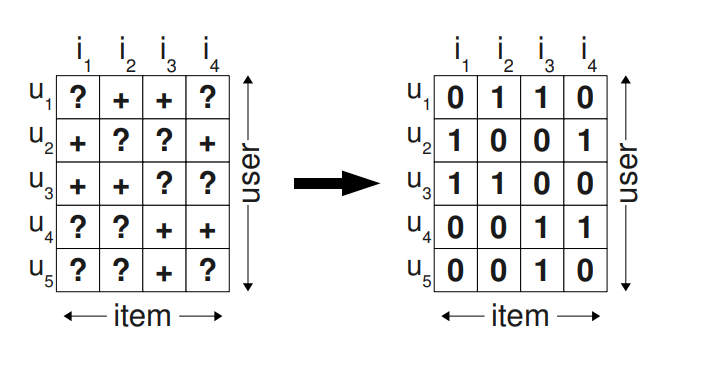
\includegraphics[max width=10cm,max height=10cm,keepaspectratio]{img_2_8}
	\caption[Matricea de interacțiuni]{Matricea de interacțiuni, mulțimea $S$. Imagine preluată din \hyperlink{SteffenRendleChristophFreudenthalerZenoGantnerLarsSchmidtThieme}{[9]}.}
\end{figure} 

O abordarea uzuală pentru recomandarea de articole este să fie estimat scorul $\hat{x}_{ui}$ care să reflecte preferința utilizatorului $u$ pentru articolul $i$. Apoi fiecare articol primește un rang după sortarea scorurilor.

Setul de antrenare (vezi figura 2.4) este definit de mulțimea $D_S := \{(u,i,j)|i \in I_u^+ \wedge j \in I \setminus I_u^+\}$ unde $(u,i,j)$ înseamnă că utilizatorul $u$ preferă articolul $i$ în detrimentul articolului $j$.
\begin{figure}[!h]
	\centering
	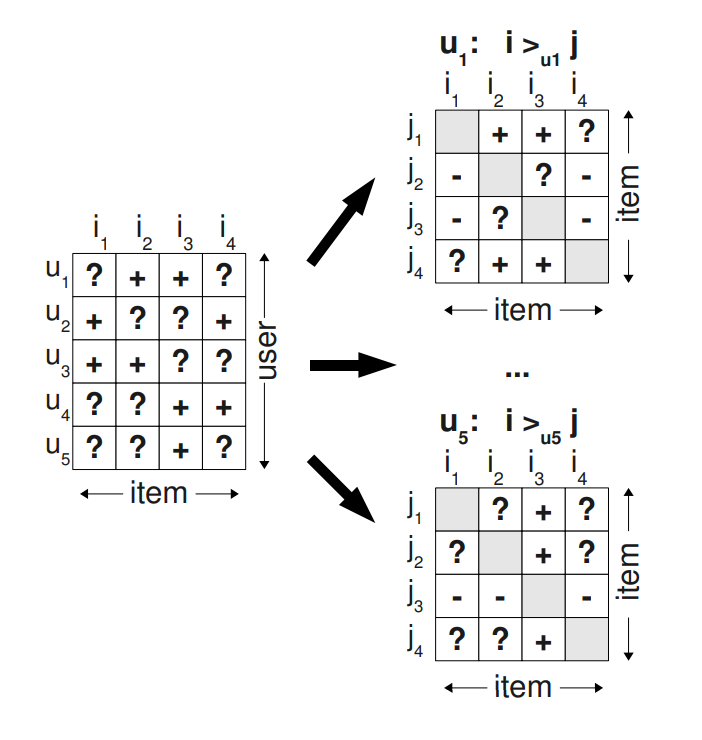
\includegraphics[max width=10cm,max height=10cm,keepaspectratio]{img_2_9}
	\caption[Setul de antrenare]{Setul de antrenare. $+$ reprezintă articolele $i$ pe care utilizatorul le preferă în locul articolelor $j$, $-$ utilizatorul preferă articolele $j$ în loc de $i$, iar $?$ reprezintă lipsa informației despre acea interacțiune. Imagine preluată din \hyperlink{SteffenRendleChristophFreudenthalerZenoGantnerLarsSchmidtThieme}{[9]}.}
\end{figure} 

Criteriul de optimizare pentru pentru rangurile personalizate este definit după cum urmează:
\begin{align}
	BPR-OPT := \sum_{(u,i,j) \in D_S} \ln{\sigma(\hat{x}_{uij})} - \lambda_\Theta||\Theta||^2
\end{align}
unde $\sigma$ este funcția sigmoid, $\sigma(x) := \frac{1}{1+e^{-x}}$, $\Theta$ reprezintă vectorul parametru al modelului care definește interacțiunea dintre utilizatorul $u$, articolul $i$ și articolul $j$, iar $\lambda_\Theta$ reprezintă parametrii de regularizare.

Cu aceste definiți putem defini și procedura de învățare a $BPR$ după cum urmează în figura 2.5:
\begin{figure}[!h]
	\centering
	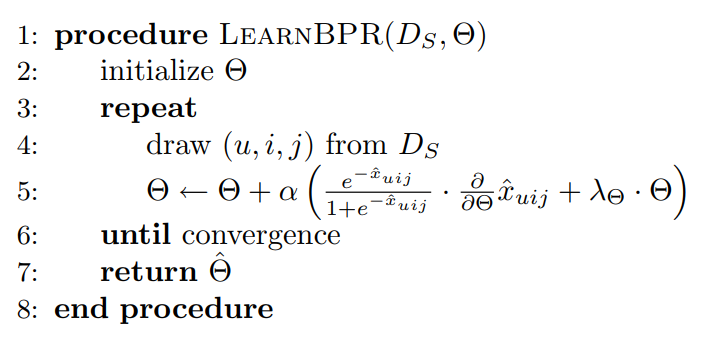
\includegraphics[max width=10cm,max height=10cm,keepaspectratio]{img_2_10}
	\caption[Procedura de învățarea BPR]{Optimizarea modelului bazată metoda gradientului descendent cu parametrul de învățare $\alpha$ și regularizarea $\lambda_\Theta$. Imagine preluată din \hyperlink{SteffenRendleChristophFreudenthalerZenoGantnerLarsSchmidtThieme}{[9]}.}
\end{figure}

\vspace{5mm}
\subsubsection*{WARP: Weighted Approximate-Rank}

Această metodă își are originile în procesarea imaginilor și anume pentru un set de reprezentări ale unor imagini $x \in R^d$ și pentru un set de reprezentări ale unor adnotări $i \in \Upsilon = \{1, ..., Y\}$ - inidici intr-un dicționar cu posibile adnotări, metoda învață să mapeze imagini din spațiul reprezentărilor într-un spațiu comun $R^D$
\begin{align}
	\Phi_{I}(x):R^d \rightarrow R^D
\end{align}
în același timp învățând și mapări pentru adnotări în același spațiu
\begin{align}
	\Phi_{W}(i):{1,...,Y} \rightarrow R^D
\end{align}

Scopul principal fiind acela de a oferi ranguri posibilelor adnotări pentru o imagine dată astfel încât cel mai mare rang să descrie cel mai bine conținutul semnatic al imaginii. 

Modelul folosit este definit în continuare:
\begin{align}
	f_{i}(x) = \Phi_{W}(i)^T \Phi_{I}(x)
\end{align}

Metoda învață să producă ranguri optimizate pentru primele adnotări din listă, ceea ce înseamnă că optimizează precizia@k.

În ceea ce privește funcția de eroare definim: $f(x) \in R^Y$ ce produce un scor pentru fiecare etichetă și unde $f_i(x)$ este valoarea etichetei $i$. Definim funcția de eroare pentru ranguri ca fiind:
\begin{align}
	err(f(x),y) = L(rank_y(f(x)))
\end{align}
unde $rank_y(f(x))$ este rangul etichetei corecte data de $f(x)$:
\begin{align}
	rank_y(f(x)) = \sum_{i \neq y}I(f_i(x) \geq f_y(x))
\end{align}
unde I este funcția indicator, iar $L(\cdot)$ transformă rangul în penalizare
\begin{align}
	L(k) = \sum_{j=1}^k\alpha_j, \quad cu \quad \alpha_1 \geq \alpha_2 \geq ... \geq 0.
\end{align}

$L(\cdot)$ poate lua diferite forme în funcție de ce se dorește a optimiza: $\alpha_j=\frac{1}{Y-1}$ optimizează rangul mediu, $\alpha_j=1$ și $\alpha_{j>1}=0$ optimizează proporția de ranguri corecte aflate în top, iar valorile mari ale lui $\alpha$ optimizează primele $k$ în lista de ranguri\hyperlink{JasonWestonSamyBengioNicolasUsunier}{[8]}.

Cu definițiile prezentate mai sus putem descrie algoritmul acestei metode după cum urmează.
\begin{figure}[!h]
	\centering
	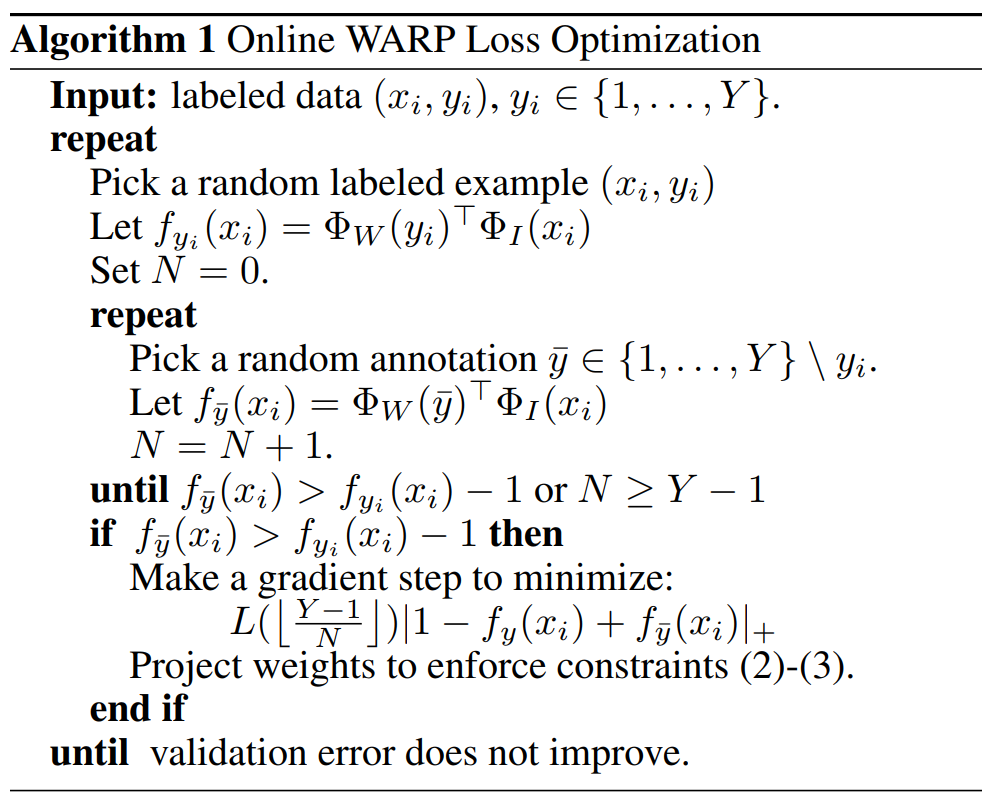
\includegraphics[max width=10cm,max height=10cm,keepaspectratio]{img_2_7}
	\caption[Online WARP Loss Optimization]{Online WARP Loss Optimization. Imagine preluată din \hyperlink{JasonWestonSamyBengioNicolasUsunier}{[8]}.}
\end{figure} 

\vspace{5mm}
\subsubsection*{k-OS WARP}
De completat ...

\section{Modelul LightFM}


\section{Rețele neurale convoluționale}

\subsection{Noțiuni generale}

Rețelele neurale convoluționale sunt rețelele formate din neuroni ce învață ponderi ($w$) și baiasuri ($b$). Scopul rețelei convoluționale este de a primi o imagine la input și de a scoate la output un scor pentru fiecare clasă ce corespunde imaginii. 

Spre exemplu, la input se dă o imagine cu un autovehicul, iar rețeaua convoluțională poate spune că în imagine este o mașină în proporție de 80\%, un camion în proporție de 10\%, un avion în proporție de 6\%, o barcă în proporție de 3\% sau un cal în proporție de 1\%.
\begin{figure}[!h]
	\centering
	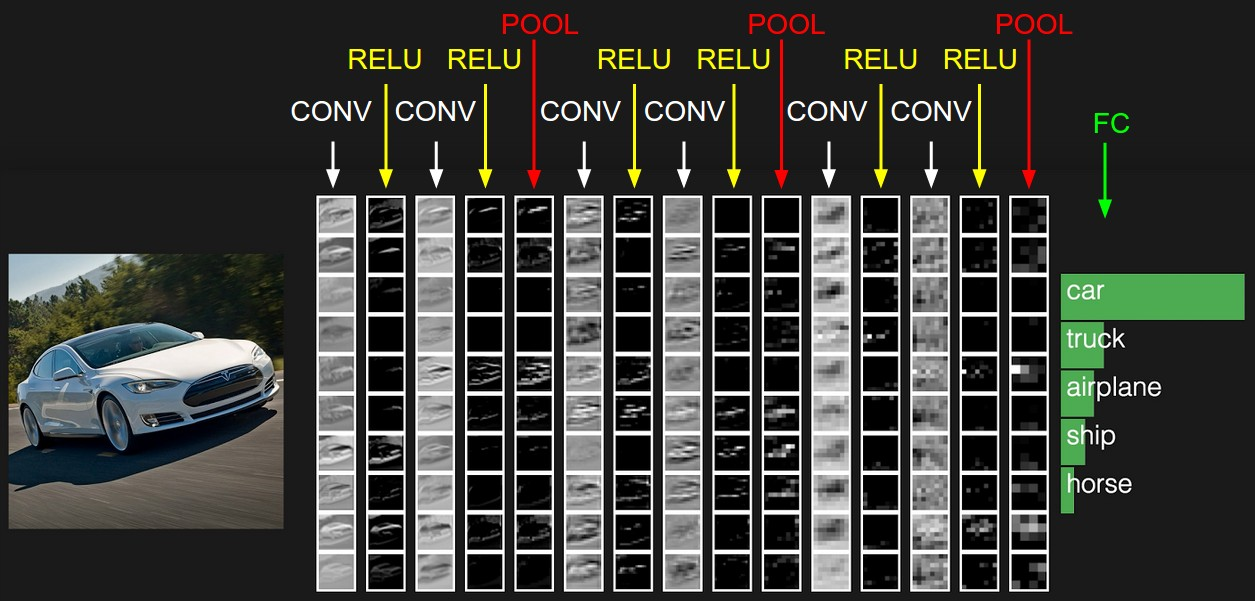
\includegraphics[max width=10cm,max height=10cm,keepaspectratio]{img_2_3}
	\caption[Exemplu rețea convoluțională]{Exemplu de rețea convoluțională care primește la input o imagine și produce la output o listă de clase ce pot descrie imaginea de input. Imagine preluată din \hyperlink{datameetsmedia}{[7]}.}
\end{figure} 

Rețelele convoluționale sunt compuse dintr-o secvență de straturi ce poate fi împărțită în trei tipuri principale \hyperlink{cs231n}{[7]}:
\begin{enumerate}
  \item Stratul convoluțional este stratul de bază într-o rețea. Parametrii acestui strat sunt reprezentați de filtre învățabile, unde fiecare filtru reprezintă o mică bucată din imaginea de input. De exemplu, un filtru pentru acest strat poate avea dimensiunea de $5 \times 5 \times 3$, dimensiune ce reprezintă faptul că se iau 5 pixeli pe lațime, 5 pixeli pe înălțime și o adâncime de 3 pixeli, unde adâncimea reprezintă canalele RGB. În continuare se glisează fiecare filtru peste input și se compune produsul dintre filtre și input la fiecare poziție. În urma acestei operații se produce un vector de activare 2-dimensional care reprezintă răspunsul filtrului la fiecare poziție. Altfel spun, rețeaua va învăța filtre care se activează atunci când sunt prezente anumite tipuri de caracteristici, precum culoarea sau orientarea (vezi figura 2.8).
\begin{figure}[!h]
	\centering
	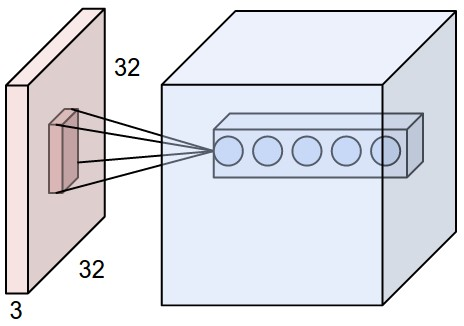
\includegraphics[max width=10cm,max height=10cm,keepaspectratio]{img_2_4}
	\caption[Exemplu de filtru aplicat peste input]{Exemplu de filtru aplicat peste input într-un strat convoluțional. Imagine preluată din \hyperlink{datameetsmedia}{[7]}.}
\end{figure}   
  
  \item Stratul de pooling reprezintă o practică des folosită între mai multe straturi convoluționale succesive. Această operație reduce numărul de parametrii (dimensiunea modelului), computațiile din rețea și controlează overfittingul. Se execută indepedent pe fiecare nivel al adâncimii unui input și pastrează valoarea maximă a acelei zone (de cele mai multe ori). Rezultatul este o zonă de caracteristicii mai mică dar care păstrează cea mai relevantă statistică (vezi figura 2.9).
\begin{figure}[!tbp]
  \begin{subfigure}[b]{0.4\textwidth}
    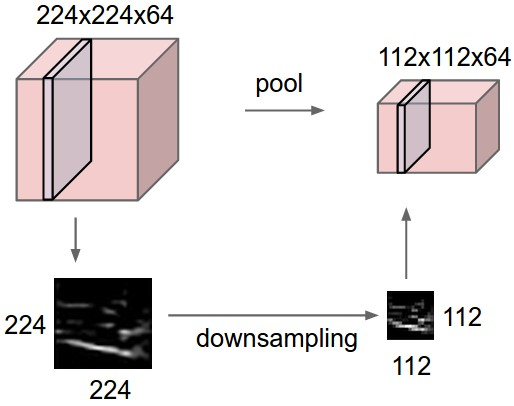
\includegraphics[width=\textwidth]{img_2_5}
    \caption{Reducerea dimensiunii.}
    \label{fig:f1}
  \end{subfigure}
  \hfill
  \begin{subfigure}[b]{0.4\textwidth}
    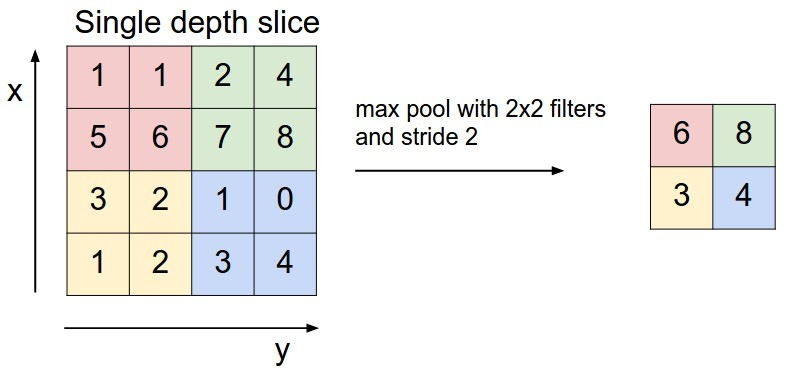
\includegraphics[width=\textwidth]{img_2_6}
    \caption{Filtrul de $2\times2$ aplicat ce păstrează valoarea maximă.}
    \label{fig:f2}
  \end{subfigure}
  \caption[Exemplu de pooling]{Exemplu de pooling. Imagine preluată din \hyperlink{datameetsmedia}{[7]}.}
\end{figure}
  
  \item Fully-Connected Layer este stratul în care caracteristicile sunt vectorizate pentru a putea fi folosite.
\end{enumerate}

\subsection{VGG}

VGG este o arhitectură clasică de rețea cu filtre convoluționale foarte mici, de dimensiune $3 \times 3$ și care poate avea un număr a straturilor de ponderi de 16 - 19. 

În ceea ce privește arhitectura (vezi figura 2.10), inputul în rețeaua convoluțională este de dimensiune fixă și anume $224 \times 224$ imagine RGB. Mai departe, imaginea este trecută printr-un set de straturi convoluționale unde sunt utilizate filtre de dimensiune mică, $3 \times 3$ - fiind cea mai mică dimensiune ce poate captura noțiunile de stânga/dreapta, sus/jos sau centru. Într-una dintre configurații se utilizează un filtru convoluțional de dimensiune $1 \times 1$. Pasul în straturile convoluționale este fixat la 1 pixel.

Poolingul este compus din cinci straturi de max-pooling care urmează după unele straturi convoluționale. Max-poolingul este calculat cu ferestre de $2\times2$ pixel și cu pas de 2 pixeli.

Odată trecută imaginea prin straturile convoluționale și cele de pooling ajunge în trei straturi fully-connected. Primele două straturi au câte 4096 de canale fiecare, iar al treilea are 1000 de canale. Canalele celui de-al treilea strat sunt asociate claselor, fiecare canal reprezintă o clasă.

Ultimul strat din rețea este un strat soft-max \hyperlink{SimonyanKarenZissermanAndrew}{[10]}.

\begin{figure}[!h]
	\centering
	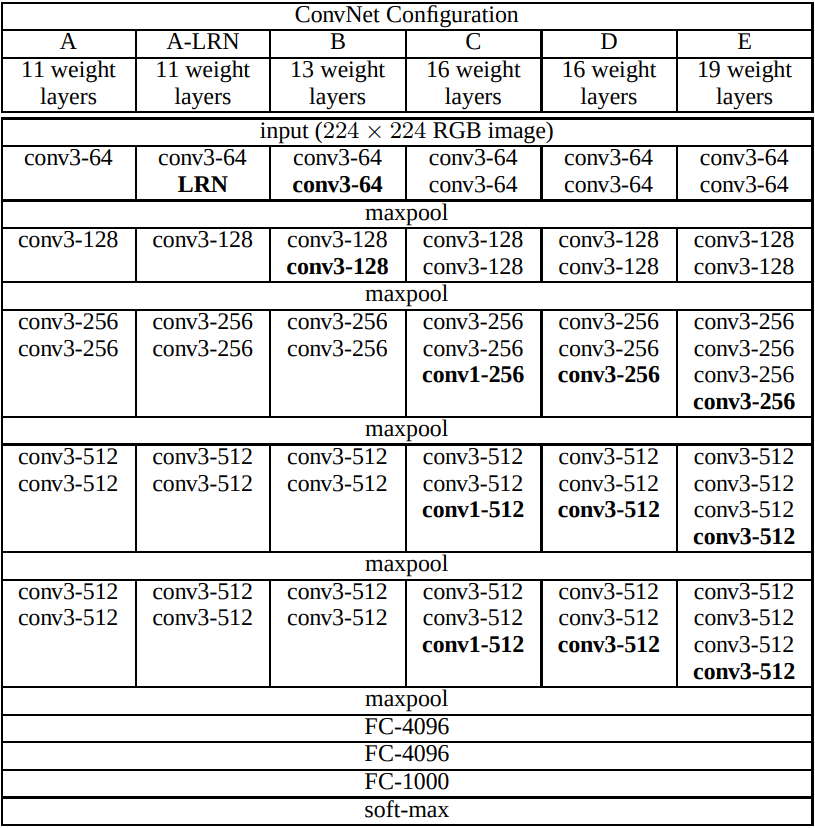
\includegraphics[max width=12cm,max height=12cm,keepaspectratio]{img_2_11}
	\caption[Configurații VGG]{Configurații ale rețelei VGG. Imagine preluată din \hyperlink{SimonyanKarenZissermanAndrew}{[10]}.}
\end{figure}   

\subsection{InceptionV3}
Prima arhitectura de Inception a apărut sub numele de GoogLeNet. O a doua versiune de Inception a fost definită prin introducerea de batch-uri normalizate. Iar mai apoi, versiunea a treia în care a fost adăugate idea de factorizare.

Factorizarea în filtre convoluționale mici (vezi figura 2.11) presupune înlocuirea stratului cu filtru de dimensiune $5 \times 5$ cu două straturi de dimensiune $3 \times 3$ astfel reducânduse dimensiunea de la $5 \times 5 = 25$ la $3 \times 3 + 3 \times 3 = 18$.
\begin{figure}[!h]
	\centering
	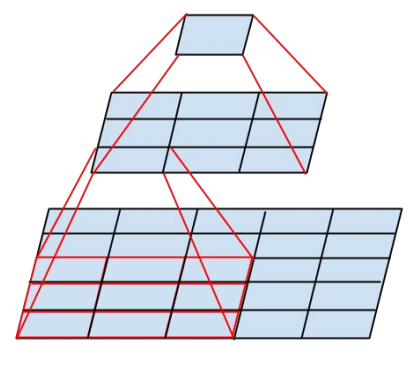
\includegraphics[max width=7cm,max height=7cm,keepaspectratio]{img_2_17}
	\caption[Factorizarea în filtre convoluționale mici]{Factorizarea în filtre convoluționale mici. Filtrul de dimensiune $5 \times 5$ înlocuit cu două de dimensiune $3 \times 3$. Imagine preluată din \hyperlink{guideinceptionv3}{[14]}.}
\end{figure}   

Factorizarea spațială în convoluții asimetrice (vezi figura 2.12) presupune înlocuirea stratului cu filtru de dimensiune $3 \times 3$ cu două straturi de dimensiune $3 \times 1$ și $1 \times 3$ astfel reducânduse dimensiunea de la $3 \times 3 = 9$ la $3 \times 1 + 1 \times 3 = 6$. 
\begin{figure}[!h]
	\centering
	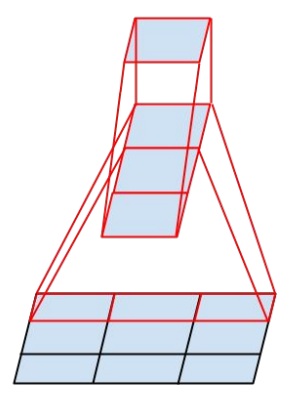
\includegraphics[max width=7cm,max height=7cm,keepaspectratio]{img_2_18}
	\caption[Factorizarea spațială în convoluții asimetrice]{Factorizarea în filtre convoluționale mici. Filtrul de dimensiune $3 \times 3$ înlocuit cu două de dimensiune $3 \times 1$ și $1 \times 3$.  Imagine preluată din \hyperlink{guideinceptionv3}{[14]}.}
\end{figure}

Clasificatorul auxiliar (vezi figura 2.13) este utilizat în InceptionV3 ca regulizator și este poziționat în partea superioară a utimelor $17 \times 17$ straturi. Batch-urile normalizate sunt de asemeanea folosite în clasificatorul auxiliar.
\begin{figure}[!h]
	\centering
	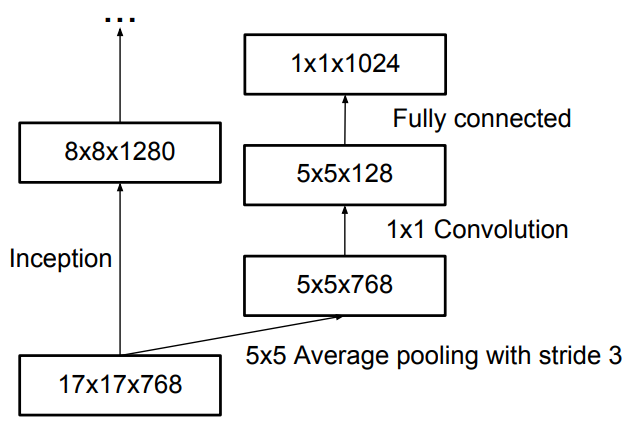
\includegraphics[max width=10cm,max height=10cm,keepaspectratio]{img_2_19}
	\caption[Clasificator auxiliar]{Clasificatorul auxiliar. Imagine preluată din \hyperlink{guideinceptionv3}{[14]}.}
\end{figure}

Reducerea eficientă a dimensiunii (vezi figura 2.14) se face prin utilizarea a două blocuri paralele, fie P și C. Primul dintre acestea, P, fiind un strat de activare de pooling (media sau maxim pooling). Ambele straturi au filtre cu pas 2 care sunt concatenate.
\begin{figure}[!h]
	\centering
	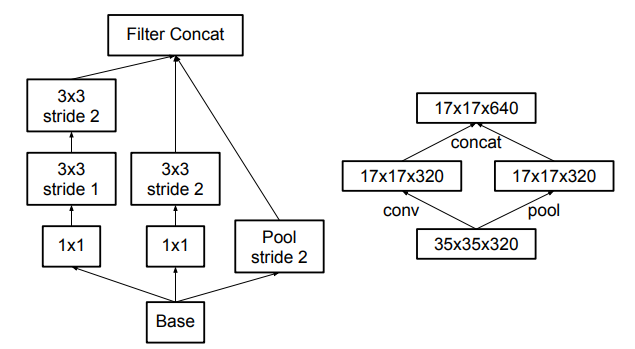
\includegraphics[max width=17cm,max height=12cm,keepaspectratio]{img_2_20}
	\caption[Reducerea eficientă a dimensiunii]{Modulul care reduce dimensiunea. Diagrama din dreapta reprezintă aceași soluție însă din perspectiva dimensiunii rețelei. Imagine preluată din \hyperlink{guideinceptionv3}{[14]}.}
\end{figure}   

Arhitectura completă este prezentată în figura 2.15.
\begin{figure}[!h]
	\centering
	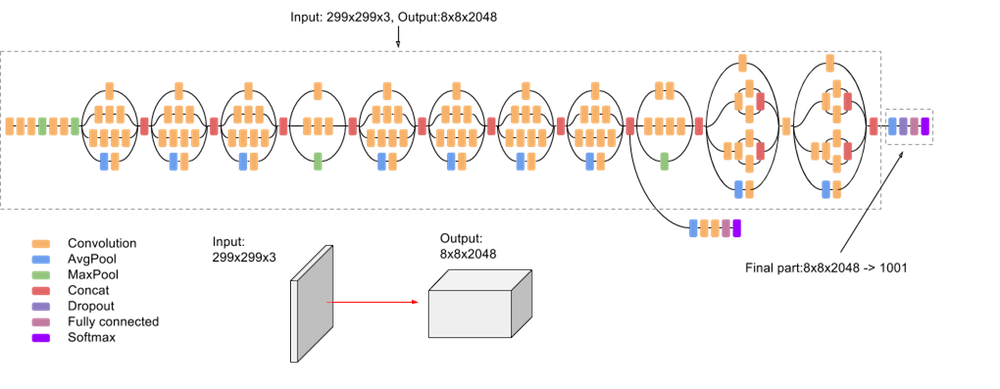
\includegraphics[max width=17cm,max height=12cm,keepaspectratio]{img_2_16}
	\caption[Arhitectura InceptionV3]{Arhitectura rețelei InceptionV3. Imagine preluată din \hyperlink{guideinceptionv3}{[14]}.}
\end{figure}   


\subsection{ResNet}
Fie $H(x)$ maparea de bază unde $x$ reprezintă inputul. Funcția reziduală poate fi aproximată cu $F(x) := H(x) - x$, maparea de bază fiind $F(x) + x$.

\begin{figure}[!h]
	\centering
	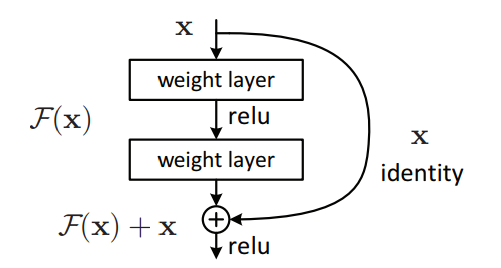
\includegraphics[max width=10cm,max height=10cm,keepaspectratio]{img_2_12}
	\caption[Învățarea reziduală]{Învățarea reziduală. Imagine preluată din \hyperlink{KaimingHeXiangyuZhangShaoqingRenJianSun}{[11]}.}
\end{figure}  

Învățarea reziduală se aplică la câtva grupuri de straturi. Putem defini un bloc de straturi ca fiind 
\begin{align}
	y = F(x,\{W_i\}) + x
\end{align}
unde $x$ și $y$ reprezintă inputul și outputul straturilor considerate. Funcția $F(x, \{W_i\})$ reprezintă maparea reziduală ce trebuie învățată.

Dimensiunea lui $x$ și $F$ din ecuația de mai sus trebuie să fie egale. Redefinim ecuația după cum urmează
\begin{align}
	y = F(x,\{W_i\}) + W_sx
\end{align}
unde $W_s$ este o proiecție liniară a scurtăturilor conexiunilor pentru ca dimensiunile să se potrivească.

ResNet (vezi figura 2.17) pleacă de la o rețea simplă. Rețeaua simplă fiind inspirată de rețeaua VGG. Straturile convoluționale au în general filtre de dimensiune $3 \times 3$ și se bazează de două reguli de design: - pentru outputuri cu același număr de caracteristici, straturile vor avea același număr de filtre; - dacă numărul de caracteristicii este injumătățit, numărul de filtre este dublat astfel încât să fie păstrată complexitatea de timp pe strat.

Poolingul se realizează dupa straturile convoluționale cu un pas de 2 pixeli. Rețeaua se termină cu un strat de pooling mediu și un strat fully-connected softmax cu 1000 de canale.

Bazată pe rețeaua descrisă mai sus, rețeaua reziduală presupune inserția unor scurtături. Scurtăturile identice (vezi formula 2.8) pot fi direct utilizate când inputul și outputul au aceași dimensiune. Când dimensiunea crește considerăm două opțiuni: - scurtătura calculează în continuare maparea identității. Această opțiune nu introduce parametrii noi; - proiecția scurtăturii din formula 2.9 este utilizată pentru a potrivi dimensiunile. În ambele situații când se folosesc scurtăturile pentru pentru a sări peste două straturi sunt calculate cu un pas de 2 pixeli.

\begin{figure}[!h]
	\centering
	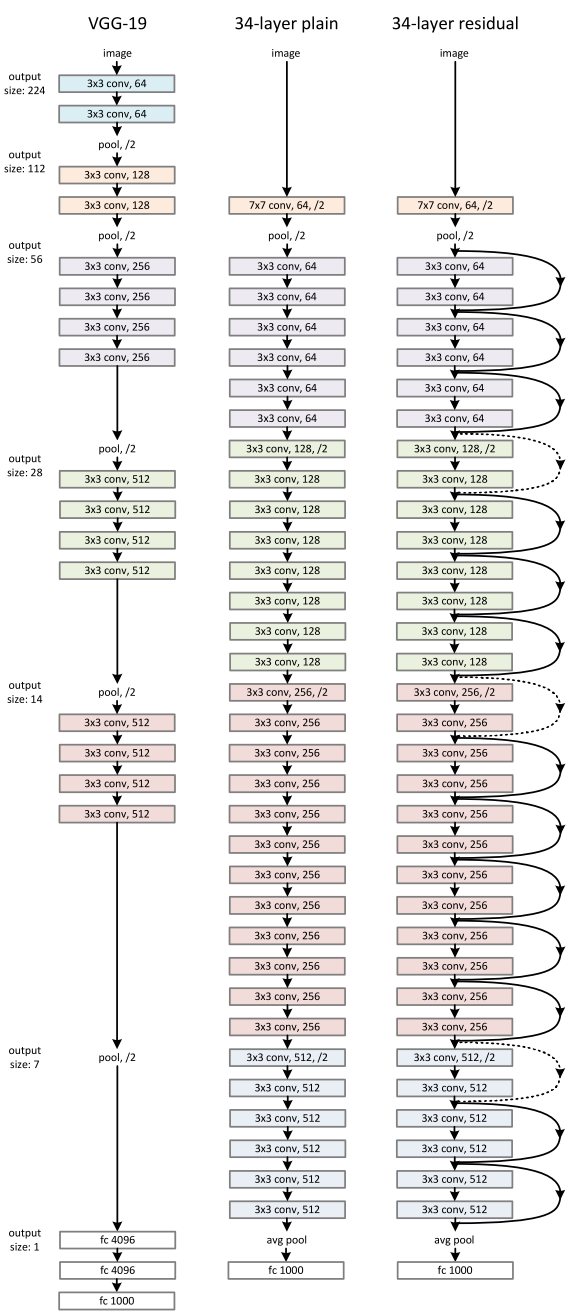
\includegraphics[max width=10cm,max height=20cm,keepaspectratio]{img_2_13}
	\caption[Rețeaua ResNet]{Prima rețea (stânga) este o rețea VGG19. A doua rețea (centru) este o rețea simplă cu 34 de straturi. A treia rețea (dreapta) este o rețea reziduală cu 34 de straturi. Imagine preluată din \hyperlink{KaimingHeXiangyuZhangShaoqingRenJianSun}{[11]}.}
\end{figure}  

\subsection{NASNet}
NASNet este o arhitectură de rețea bazată pe tehnica de căutare Neural Architecture Search (NAS, figura 2.18). NAS presupune un controler cu o rețea neurală recurentă care conține mai multe rețele copii cu arhitecturi diferite. Rețelele copii sunt antrenate să conveargă pentru a obține o anumită precizie pe un set de antrenare. Rezultatele sunt utilizate pentru a actualiza controlerul ceea ce înseamnă că acest controler va genera arhitecturi mai bune în timp.
\begin{figure}[!h]
	\centering
	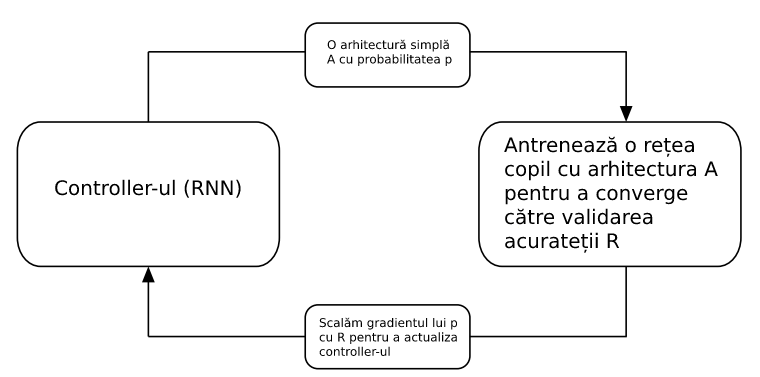
\includegraphics[max width=10cm,max height=20cm,keepaspectratio]{img_2_14}
	\caption[NAS]{Privire de ansamblu asupra unei Neural Architecture Search. Imagine preluată din \hyperlink{Zoph2018LearningTA}{[13]}.}
\end{figure}  

Plusul principal pe care îl aduce rețeaua NASnet este reprezentat de proiectarea unui nou spațiu de căutare astfel încât cea mai bună arhitectură pe setul de date CIFAR-10 poate scala către rezoluții ale imaginilor cât mai mari într-un interval definit. Astfel, acest spațiu poartă numele de \textit{NASNet search space}. În abordarea NASNet, arhitecturile rețelelor convoluționale sunt manual predeterminate, fiind compuse din celule convoluționale repetate de multe ori unde, fiecare celulă convoluțională are aceași arhitectură dar ponderi diferite.

Pentru a construi mai ușor arhitecturi scalabile pentru imagini de orice dimensiune este nevoie de două tipuri de celule convoluționale pentru a îndeplini două funcții principale: - celule convoluționale care returnează o hartă de caracteristici cu aceași dimensiune. Acest tip de celule se numește \textit{Celulă Normal}; - celule convoluționale care returnează o hartă de caracteristici cu înălțimea și lungimea harții divizată cu un factor doi. Acest tip de celule se numește \textit{Celulă de reducere} (vezi figura 2.19).
\begin{figure}[!h]
	\centering
	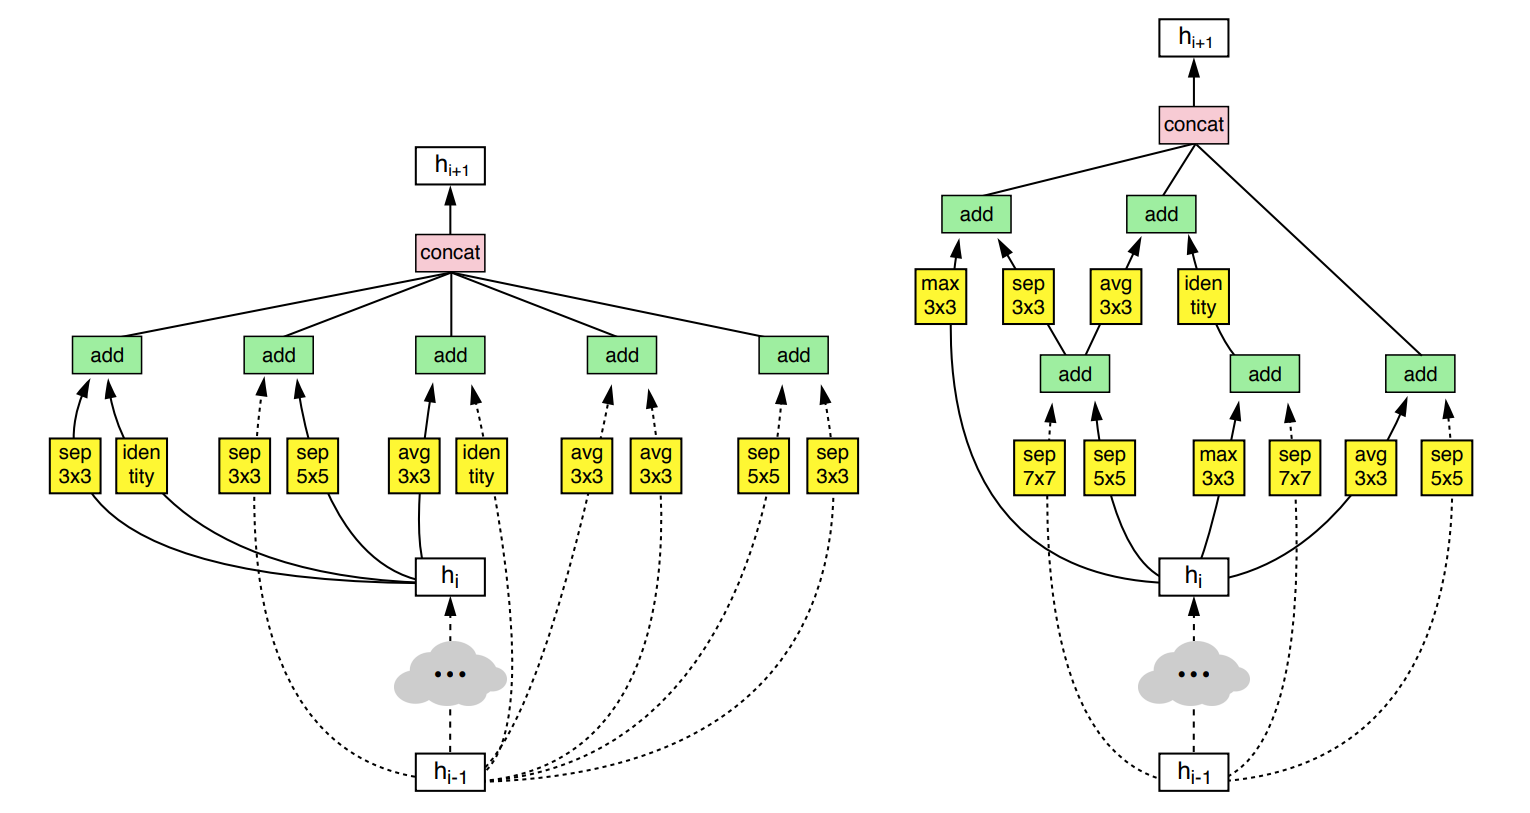
\includegraphics[max width=17cm,max height=17cm,keepaspectratio]{img_2_15}
	\caption[Celule normale și de reducere]{Celule normale (dreapta). Celule de reducere (stânga). Imagine preluată din \hyperlink{Zoph2018LearningTA}{[13]}.}
\end{figure}  

\section{Clustere}

\subsection{Noțiuni generale}

Clusterizarea este un proces de grupare a unor articole în sensul în care articolele din același cluster sunt foarte similare între ele din punct de vedere al caracteristicilor. Această metodă este des utilizată în data mining, analiza datelor, machine learning, recunoașterea tiparelor sau regăsirea informației. Există mai multe tipuri de algoritmi de clusterizare, însă, ideea de bază este aceași: clusterele sunt grupuri cu distanțe foarte mici între membrii grupului (fie distanța euclidiană, de exemplu).
\begin{figure}[!h]
	\centering
	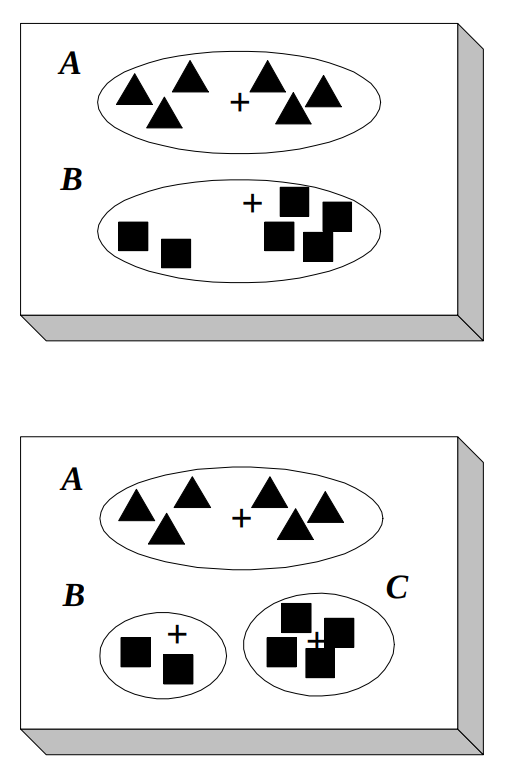
\includegraphics[max width=10cm,max height=10cm,keepaspectratio]{img_2_21}
	\caption[Exemplu clustere]{Exemplu de două clustere (sus). Exemplu de trei clustere (jos). Imagine preluată din \hyperlink{dataclusteringtechniques}{[15]}.}
\end{figure}  

Procesul de clustering poate fi împărțit în etape după cum urmează \hyperlink{dataclusteringtechniques}{[15]}:
\begin{enumerate}
	\item Colectarea datelor: alegerea articolelor pentru care se va aplica clusterizarea;
	\item Screening-ul inițial: presupune extragerea caracteristicilor relevante pentru fiecare articol din dataset;
	\item Reprezentarea: presupune pregătirea datelor pentru a putea fi folosite de către algoritmul de clusterizare, tot aici alegânduse și măsura de similaritate;
	\item Tendința de grupare: se verifică dacă datele au o tendință naturală de grupare; poate fi sărită pentru baze de date mari;
	\item Strategia de clusterizare: se alege algoritmul de clusterizare și parametrii inițiali;
	\item Validarea: se evaluează manual/vizual sau prin alte metode definite rezultatele obținute în urma clusterizări;
	\item Interpretarea: în această se compară rezultatele pe mai multe clustere, combinații de clustere și se trag concluziile.
\end{enumerate}

\subsection{K-nearest neighbors}
KNN reprezintă un model de clasificare simplu și eficient în multe cazuri. Pentru ca un articol $t$ să fie clasificat sunt căutați cei mai propiați $k$ vecini formând regiunea lui $t$. Cei mai apropiați veci sunt căutați cu o măsură de similaritate, de obicei distanța euclidiană sau similaritatea cosinus. Votul majoritar din acea regiune este folosit pentru a decide clasificarea lui $t$. $k$-ul este valoarea de care depinde destul de mult rata de succes a calsificării, cea mai simplă metodă de a alege un $k$ optim fiind reprezentată de rularea algoritmului pentru mai multe valori ale lui și observarea evoluției rezultelor.

\vspace{5mm}
Fie $D$ o colecție de $n$ clase cunoscute $\{d_1, d_2,..., d_n\}$. $Sim(d_i)$ - similaritatea celui mai indepărtat punct din regiunea locală, $N(d_i)$ - numărul de puncte din interiorul unei regiuni locale. Algoritmul de construcție al modelului este definit după cum urmează \hyperlink{gongdeguo}{[16]}:
\begin{enumerate}
	\item selectăm o măsură de similaritate și creem o matrice de similaritate peste baza de date de antrenare;
	\item setăm toate datele cu eticheta neclasificate;
	\item pentru fiecare intrare cu eticheta de neclasificat căutăm cea mai mare regiune locală care acoperă cel mai mare număr de vecini cu aceași categorie.
	\item căutam intrarea $d_i$ cu cea mai mare regiune $N_i$ printre toate regiunile locale și creem o reprezentare $<Cls(d_i), Sim(d_i), Num(d_i), Rep(d_i)>$ în modelul $M$ pentru a reprezenta toate intrările acoperite de regiunea $N_i$ și setăm etichete pentru toate aceste intrări;
	\item repetăm pași 3 și 4 până când toate intrările din baza de date de antrenare au fost clasificate;
	\item modelul $M$ este format din toate reprezentările setate în procesul de învățatare descris mai sus.
\end{enumerate}

Algoritmul de clasificare este definit după cum urmează:
\begin{enumerate}
	\item pentru ca o nouă intrare $d_t$ să fie clasificată, calculăm similaritatea ei cu toate celelalte reprezentări din model;
	\item dacă $d_t$ este acoperit doar de o reprezentare $<Cls(d_j), Sim(d_j), Num(d_j), Rep(d_j)>$ în sensul că distanța de la $d_t$ la $d_j$ este mai mică decât $Sim(d_j)$, $d_t$ este astfel clasificat ca făcând parte din clasa lui $d_j$;
	\item dacă $d_t$ este acoperit de două sau mai multe clase, clasificăm $d_t$ ca făcând parte din reprezentarea cu cea mai mare valoare a $Num(d_j)$, adică regiunea care acoperă cel mai mare număr de intrări din baza de date de antrenare;
	\item dacă nu există nicio reprezentare în modelul M care să acopere $d_t$, clasificăm $d_t$ cu o clasă nouă.
\end{enumerate}

Un exemplu vizual de execuție a algoritmului de kNN, parcurs pas cu pas, este prezentat în figura 2.21. Exemplu conține 36 de intrări din 2 clase marcate prin pătrat și cerc. Datele de test sunt reprezentate prin tringhiuri.
\begin{figure}[!tbp]
  \begin{subfigure}[b]{0.4\textwidth}
    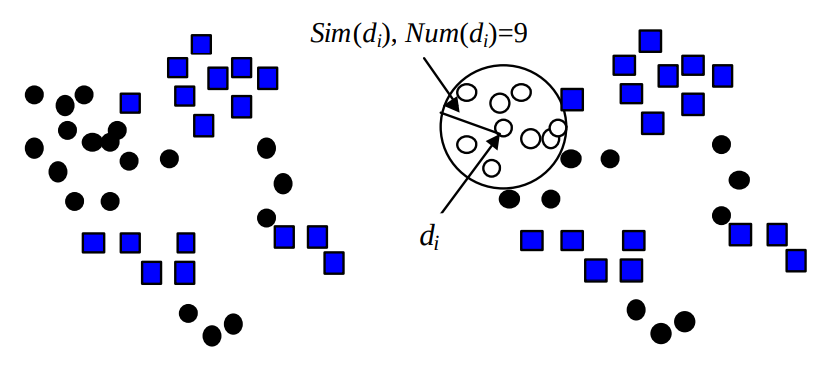
\includegraphics[width=\textwidth]{img_2_22}
    \caption{Distribuția inițială a datelor (stânga) și prima reprezentare obținută (dreapta)}
    \label{fig:f1}
  \end{subfigure}
  \hfill
  \begin{subfigure}[b]{0.4\textwidth}
    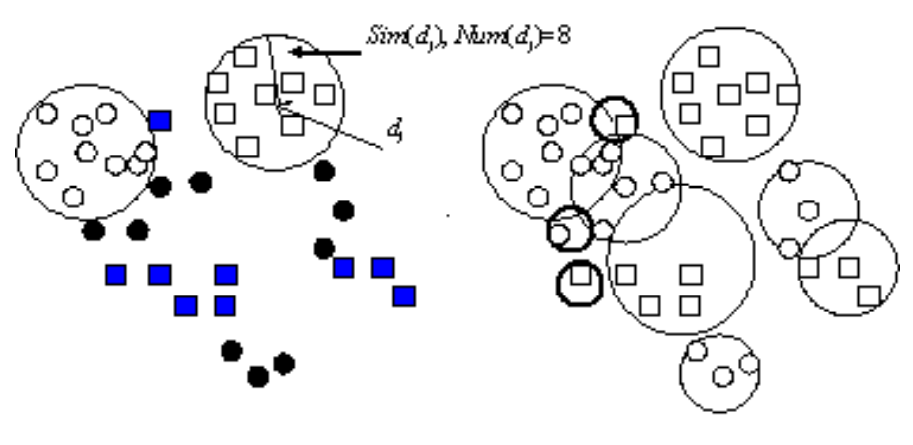
\includegraphics[width=\textwidth]{img_2_23}
    \caption{A doua reprezentare obținută (stânga) și modelul înainte de triere (dreapta)}
    \label{fig:f2}
  \end{subfigure}
  \hfill
  \begin{subfigure}[b]{0.4\textwidth}
    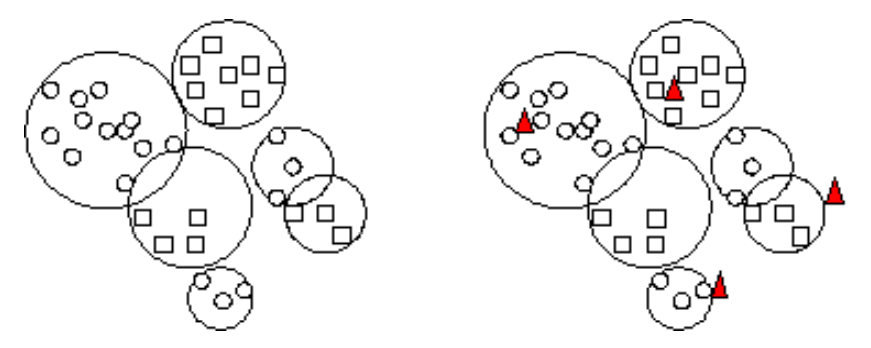
\includegraphics[width=\textwidth]{img_2_24}
    \caption{Modelul după triere (stânga) și distribuția datelor de test (dreapta)}
    \label{fig:f3}
  \end{subfigure}
  \caption[Exemplu 1 de clasificare cu kNN]{Exemplu 1 de clasificare cu kNN. Imagine preluată din \hyperlink{gongdeguo}{[16]}.}
\end{figure}  

Un al doilea exemplu de clasificare este prezentat în figura 2.22:
\begin{figure}[!tbp]
  \begin{subfigure}[b]{0.4\textwidth}
    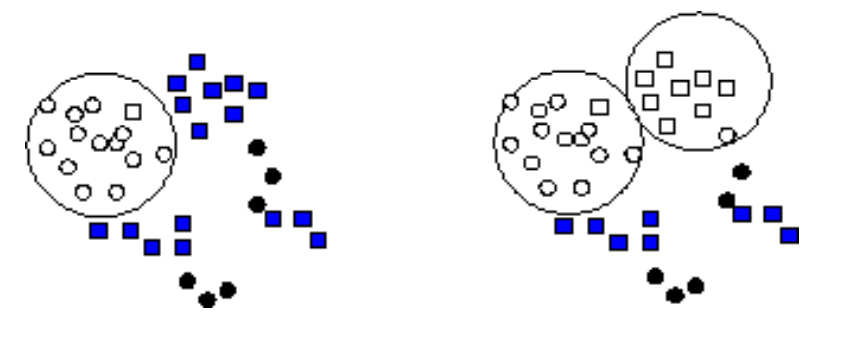
\includegraphics[width=\textwidth]{img_2_25}
    \caption{Prima reprezentare obținută (stânga) și a doua reprezentare obținută(dreapta)}
    \label{fig:f1}
  \end{subfigure}
  \hfill
  \begin{subfigure}[b]{0.4\textwidth}
    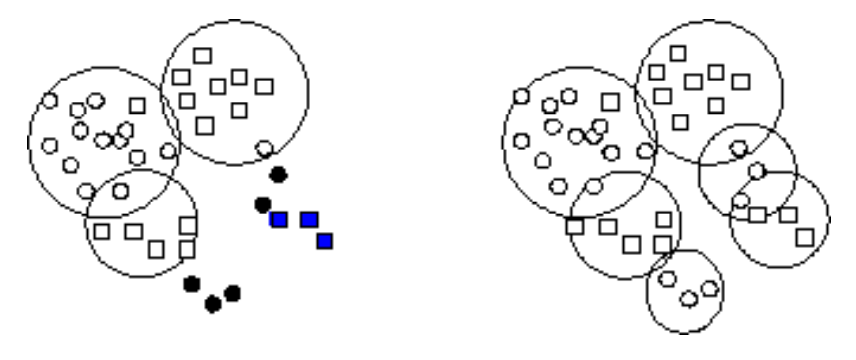
\includegraphics[width=\textwidth]{img_2_26}
    \caption{A treia reprezentare obținută (stânga) și modelul final (dreapta)}
    \label{fig:f2}
  \end{subfigure}
  \caption[Exemplu 2 de clasificare cu kNN]{Exemplu 2 de clasificare cu kNN. Imagine preluată din \hyperlink{gongdeguo}{[16]}.}
\end{figure}

\subsection{Metrici de evaluare a clusterelor}

\subsubsection{Coeficientul silhouette}

Coeficient (vezi formula 2.10) este folosit pentru a evalua clusterele în învățarea nesupervizată. Este calculat utilizând distanța euclidiană medie intra-clustere ($a$) și distanța medie către cel mai apropiat cluster ($b$) pentru fiecare intrare, adică distanța dintre o intrare și cel mai apropiat cluster din care nu face parte. Numărul de etichete trebuie să respecte constrangerea $2 \leq nr_{etichete} \leq nr_{etichete} - 1$. Valorile returnate de acest coeficient sunt cuprinse în intervalul $[-1, 1]$. Valorile apropiate de 0 indică clustere care se suprapun, valorile negative în general indică că există intrări asignate în clusterul greșit, iar valorile apropiate de 1 indică o separație bună intre clustere \hyperlink{silhouette}{[17]}.
\begin{align}
	\frac{b-a}{max(a,b)}
\end{align}


\newpage\null\newpage
\chapter{Descrierea soluției}
\section{Implementarea modelului de recomandare}
\subsection{Inițializarea}
În implementarea prezentei aplicații este folosit framework-ul de construcție a sistemelor de recomandare $LightFM$ \hyperlink{lightfm}{[21]} peste s-a construit un wrapper. 
$LightFM$ conține o implemntare în Python a unor algoritmi de recomandare atât pentru feedback implicit cât și pentru feedback explicit. Metadatele filmelor și utilizatorilor pot fi încorporate intr-un algoritm tradițional de factorizarea matricială. Reprezentarea fiecărui film și utilizator este o sumă a reprezentărilor latente ale caracteristicilor, ceea ce îi permite să generalizeze recomandările și către filme sau utilizatori noi.   

În continuare este prezentată inițializarea modelului de recomandare și explicația parametrilor folosiți atât cei definiți ca fiind maleabili cât și ceilalți parametrii puși la dispoziție de framework dar asupra cărora nu s-a intervenit în prezenta implementare:
\begin{lstlisting}[language=Python, caption=Definirea modelului de recomandare]
from lightfm import LightFM

__all__ = ['KingRec']


class KingRec(object):
    def __init__(self, no_components=50, loss='warp', learning_rate=0.05, alpha=0.02, scale=0.07):
        self.no_components = no_components
        self.loss = loss
        self.learning_rate = learning_rate
        self.item_alpha = alpha
        self.user_alpha = alpha * scale
        
        self.model = LightFM(no_components=no_components, 
        					 learning_rate=learning_rate, loss=loss,
                             item_alpha=self.item_alpha, 
                             user_alpha=self.user_alpha, 
                             random_state=2019)                       
\end{lstlisting}

Parametrii maleabili:
\begin{itemize}
  \item \textbf{no\_components}: numărul de componente reprezintă dimensiunea encodării latente a caracteristicilor utilizatorilor și filmelor. Spre exemplu, numărul de caracteristici pe fiecare utilizator este de 1000 și avem 100 de utilizatori, ceea ce înseamnă o matrice de dimensiune $100 \times 1000$. Cu numărul de componente setat la 50, cum este prezentat în fragmentul de cod de mai sus, înseamnă ca numărul caracteristicilor pe fiecare utilizator va fi redus la 50 de unde rezultă noua matrice a encodărilor latente a caracteristicilor de dimensiune $100 \times 50$.
  \item \textbf{learning\_rate}: reprezintă rata de învățare de start pe care o folosește sistemul de recomandare. Această rată se poate schimba pe parcusul rulării ca urmare a faptului că s-a folosit algoritmul de optimizare Adagrad. Mai multe detalii despre acest algoritmi au fost prezentate în capitolul 2.2.3.
  \item \textbf{loss} funcția de eroare care poate fi una dintre următoarele funcții implementate: logistic, bpr, warp, warp-kos. Mai multe detalii despre funcțiile de eroare au fost prezentate în capitolul 2.1.3.
  \item \textbf{item\_alpha} penalizarea L2 norm a caracteristicilor articolelor. Este asignată direct din parametrul $alpha$.
  \item \textbf{user\_alpha} similar cu $item\_alpha$ și este rezultatul înmulțirii dintre parametrul $alpha$ și $scale$.
  \item \textbf{random\_state}: definește starea din care pleacă modelul de recomandare și este folosită de obicei pentru o reproducere mai ușoară a acelorași rezultate de la o rulare la alta.
\end{itemize}

Alți parametrii asupra carora nu s-a intervenit în prezenta implementare:
\begin{itemize}
	\item \textbf{k}: utilizat atunci când se folosește algoritmul k-OS și reprezintă al $k$-lea exemplu pozitiv ce va fi selectat din $n$ exemple pozitive pentru fiecare utilizator. Valoarea predefinită este setată la 5.
	\item \textbf{n}: utilizat atunci când se folosește algoritmul k-OS și reprezintă numărul maxim de exemple pozitive pentru fiecare actualizare. Valoarea predefinită este setată la 10.
	\item \textbf{learning\_schedule}: reprezintă algoritmul de optimizare și poate fi unul dintre adagrad sau adadelta. În experimentele realizate în această lucrare s-a folosit valoarea predefinită din model și anume adagrad.
	\item \textbf{max\_sampled}: reprezintă numărul maxim de exemple negative folosite în antrenarea cu WARP. Valoarea predefinită este setată la 10.
\end{itemize}

Odată definit modelul de recomandare putem crea o instanță a acestuia cu parametrii doriți dupa cum urmează:
\begin{lstlisting}[language=Python, caption=Instanțierea unui model]
from kingrec import KingRec

_, learning_rate, no_components, alpha, scaling = load_params(optimized_for='auc_clusters')

king_rec = KingRec(no_components=no_components, learning_rate=learning_rate, alpha=alpha, scale=scaling, loss='warp')
\end{lstlisting}
Această instanță va fi folosită în continuare în antrenarea și evaluarea modelului.
Funcția $load\_params$ încarcă parametrii optimi pentru pentru o anumită configurație. Mai multe detalii despre această optimizare a parametrilor este prezentată în capitolul 3.4.

\subsection{Antrenarea}
Cu o instanță a unui model creată putem antrena acel model pe un set de antrenare. Pentru a încărca un set de antrenare putem folosi funcția $init\_movielens$ care încarcă datasetul pus la dispoziție de grouplens \hyperlink{movielens}{[22]}. Mai multe detalii despre structura setului de date se pot găsi în capitolul 4.1.

\begin{lstlisting}[language=Python, caption=Funcția de inițializare a bazei de date]
def init_movielens(path, min_rating=0.0, k=3, item_features=None, cluster_n=18, model='vgg19')
\end{lstlisting}
unde:
\begin{itemize}
	\item \textbf{path}: este calea către folderul cu fișierele din setul de date;
	\item \textbf{min\_rating}: este ratingul minim pentru de la care vor fi construite interacțiunile dintre utilizatori și filme. Spre exemplu, dacă setăm un rating minim de $3.5$, mulțimea interacțiunilor pozitive va fi definită de acele interacțiuni pentru care utilizatorii au acordat cel puțin un rating de $3.5$, acestea fiind considerate interacțiuni pozitive. Restul interacțiunilor sunt considerate negative;
	\item \textbf{k}: este un parametru folosit doar pentru statisticii, în contextul de față prezintă câți utilizatori au minim $k$ interacțiuni în setul de date. Valoarea $k$ este folosită în metrica de evaluare $precizie@k$ după cum este prezentat în capitolul 3.1.1; 
	\item \textbf{item\_features}: poate lua una sau mai multe valori din mulțimea ${'genres', 'clusters'}$ și descrie tipurile de metadate ale filmelor care se doresc a fi prezente în setul de date. Desigur, acest parametru poate fi omis, astfel nefiind adăugate metadate suplimentare pe lângă interacțiunile dintre utilizatori și filme.
	\item \textbf{cluster\_n}: parametru folosit doar atunci când în $item\_features$ este prezentă valoarea $clusters$ și descrie în câte clustere trebuie să fie împărțite posterele filmelor. Clusterele sunt generate în prealabil și se găsesc în path-ul menționat;
	\item \textbf{model}: specifică modelul cu care au fost create posterele. Poate fi unul dintre următoarele: vgg19, inception\_v3, resnet50.
\end{itemize}
Funcția $init\_movielens$ returnează atât setul de date de antrenare cât și pe cel de testare. De asemenea, dacă este specificat prin parametrii returnează și metadatele filmelor.

Cu setul de date încarcat, putem face antrenarea cu funcția $fit$ sau $fit\_partial$. Diferența principală dintre cele două funcții este reprezentată de faptul că $fit\_partial$ reia antrenarea din starea curentă a modelului pe când $fit$ începe dintr-o stare nouă. 

\begin{lstlisting}[language=Python, caption=Antrenarea modelului]
model = king_rec.model
model.fit(interactions=train, item_features=item_features, epochs=epochs, verbose=True, num_threads=threads)
\end{lstlisting}
unde:
\begin{itemize}
	\item \textbf{interactions}: primește interacțiunile definite dintre utilizatori și filme;
	\item \textbf{item\_features}: reprezintă metadatele filmelor, dacă este cazul;
	\item \textbf{epochs}: reprezintă numărul de epoci pentru care vrem să facem antrenarea
	\item \textbf{verbose}: dacă este setat pe $True$ afișează progresul antrenării;
	\item \textbf{num\_threads}: numărul de threaduri pe care să fie executată antrenarea.
\end{itemize}

\subsection{Evaluarea}
Pe un model antrenat vom evalua două metrici pe setul de date de testare și anume \textit{acuratețea} și \textit{precizia@k}.
Prima dintre ele, \textit{acuratețea} este definită ca fiind probabilitatea ca un exemplu pozitiv ales în mod aleator să fie clasat mai sus în recomandări decât un exemplu negativ ales în mod aleator. Cea de-a doua, \textit{precizia@k} este definită de numărul de exemple pozitive aflate în primele $k$ recomandări.

Acuratețea poate fi calculată cu funcția $auc\_score$:
\begin{lstlisting}[language=Python, caption=Acuratețea unui model]
test_auc = auc_score(model, test_interactions, item_features=item_features, num_threads=threads).mean()
\end{lstlisting}
unde:
\begin{itemize}
	\item \textbf{model}: este modelul antrenat anterior;
	\item \textbf{test\_interactions}: reprezintă interacțiunile de test create cu funcția de inițializare a bazei de date;
	\item \textbf{item\_features}: reprezintă metadatele filmelor create cu funcția de intițializare a bazei de date;
	\item \textbf{num\_threads}: numărul de threaduri pe care se va executa evaluarea modelului.
\end{itemize}
Rezultatul produs este reprezentat de un scor de acuratețe pentru fiecare utilizator din setul de antrenare, iar rezultatul final al modelului este reprezentat de $mean$-ul tuturor rezultatelor de acuratețe per utilizator.

Precizia@k poate fi calculată cu funcția $precision\_at\_k$:

\begin{lstlisting}[language=Python, caption=Precizia@k a unui model]
test_precision = precision_at_k(model, test_interactions, item_features=item_features, k=k, num_threads=threads).mean()
\end{lstlisting}
unde:
\begin{itemize}
	\item \textbf{model, test\_interactions, item\_features și num\_threads}: descrise ca mai sus;
	\item \textbf{k}: numărul de recomandări peste care se calculează precizia pentru un utilizator.
\end{itemize}
Rezultatul produs este reprezentat de un scor de precizie@k pentru fiecare utilizator din setul de antrenare, iar rezultatul final al modelului este reprezentat de $mean$-ul tuturor rezultatelor de precizie per utilizator.

\section{Clusterizarea posterelor}
Procesul de clusterizare al posterelor presupune transformarea posterelor filmelor din imagini în clustere asociate fiecărui poster. Numărul total de clustere poate varia de la 2 până la 20 în cadrul acestei aplicații. De cele mai multe ori s-au folosit 18 clustere pentru a fi mapate 1 la 1 cu genurile filmelor.

Acest proces poate fi împărțit în două etape:
\begin{enumerate}
	\item Extragerea caracteristicilor din postere: în extragerea caracteristicilor din postere se folosesc mai multe rețele preantrenate printre care VGG16, VGG19, InceptionV3, ResNet50 sau NASNet. Mai multe detalii despre rețelele preantrenate pot fi găsite în capitolul 2.4. Folosim fiecare dintre rețelele menționate anterior până la stratul de clasificare, adică fără top-ul rețelelor, pentru a ne extrage doar caracteristicile din imagini. Imaginile în toate cele cinci rețele preantrenate întră cu dimensiunea fixă de $224 \times 224 \times 3$, inclusiv în rețeaua NASNet, chiar dacă aceasta poate accepta și dimensiuni mai mari. Fiecare film are câte un set de postere asociate, după cum este prezentat în capitolul 4.2. Din aceste seturi de postere alegem pentru fiecare film doar primul poster, poster pe care îl trecem prin fiecare dintre rețelele menționate mai sus. Odată trecut prin fiecare rețea, salvăm caracteristicile aferente fiecărei rețele într-un fișier specific. Aceste fișiere sunt formate din id-ul filmului și caracteristicile extrase de rețeaua specifică din primul poster al fimului.
Funcția care se ocupă de acest proces este $extract\_images\_features()$ din modulul $extract\_features.py$.
	\item Creeare clusterelor pe baza caracteristicilor posterelor: odată create fișierele cu caracteristici pentru fiecare rețea putem rula funcția $explore\_clusters()$ din modulul $create\_clusters.py$. În acest moment fiecare fișier de caracteristici va fi parcurs, iar pentru fiecare dintre aceste fișiere vom crea între 2 și 20 de clustere. La final, toate aceste clustere vor fi salvate într-un fișier asociat rețelei preantrenate. Spre exemplu, rulam funcția de creeare clustere pentru rețeaua preantrenată vgg19. Funcția va citi din fișierul asociate rețelei caracteristicile posterelor pentru fiecare film. Cu aceste caracteristici va genera $2, 4, 6, ..., 20$ de clustere. La final toate clusterele sunt salvate într-un fișier specific rețelei sub forma: id film, id poster, cluster 2 (unde va fi trecut în care cluster dintre cele două face parte posterul curent), cluster 4 (similar cu cluster 2), ..., cluster 20 (similar cu celelalte).
\end{enumerate}

\section{Construcția bazei de date}
Pentru construcția setului de date a fost folosită clasa \textit{Dataset} din framework-ul LightFM. Prima etapă în construirea bazei de date este citirea ratingurilor date de utilizatori filmelor. Odată citite ratingurile aplicăm filtrarea de minim rating, dacă este cazul. Ratingurile astfel rămase compun matricea de interacțiune. Se face un split de $80\%$ date de antrenare și $20\%$ date de testare pe aceste interacțiuni.

Pe parte de caracteristici, se folosesc prestabilit atât pentru utilizatori cât și pentru filme matrici de identitate. Spre exemplu, daca avem 500 de utilizatori și 1000 de filme vom avea matricea de caracteristici a utilizatorilor de dimensiune $500 \times 500$ având valoarea 1 pe diagonală, iar matricea de caracteristici a filmelor de dimensiune $1000 \times 1000$, având de asemenea valorea 1 pe diagonală.

În continuare, în funcție de parametrii setați în funcția \textit{init\_movielens} se încarcă și celelalte caracterstici specifice filmelor. Dacă avem setate genurile pentru a fi încărcate în matricea de caracteristici atunci pentru fiecare film vom citi din fișierul specific genurilor din setul de date genurile acestora. Un film poate avea unul sau mai multe genuri. Pentru a introduce aceste caracteristici în matricea de caracteristici vom aplica \textit{one hot encoding} ceea ce presupune că pentru o mulțime de genuri de dimensiune $n$ vom codifica mulțimea genurilor asociate unui film într-un vector de prezență de dimensiune $n$. Ceea ce înseamnă că dacă avem o mulțime de șapte genuri, fie ele genul 1, genul 2, ..., genul 7. Dacă un film are genul 3 și genul 7 atunci vectorul lui de caracteristici asociate genurilor va fi următorul $[0, 0, 1, 0, 0, 0, 1]$.

De asemenea funcția \textit{init\_movielens} poate inițializa și clusterele aferente fiecărui film. Procesul este similar cu cel definit mai sus pentru transferul genurilor filmelor în matricea de caracteristici.

Cu cele de mai sus definite propune un exemplu ce înglobează descrierea de mai sus:
Fie un set de date cu 500 de utilizatori și 1000 de filme. Numărul total de genuri este de 18. Numărul total de clustere este corelat cu numărul total de genuri, ceea ce înseamnă că vom avea un total de 18 clustere.
\begin{figure}[!h]
	\centering
	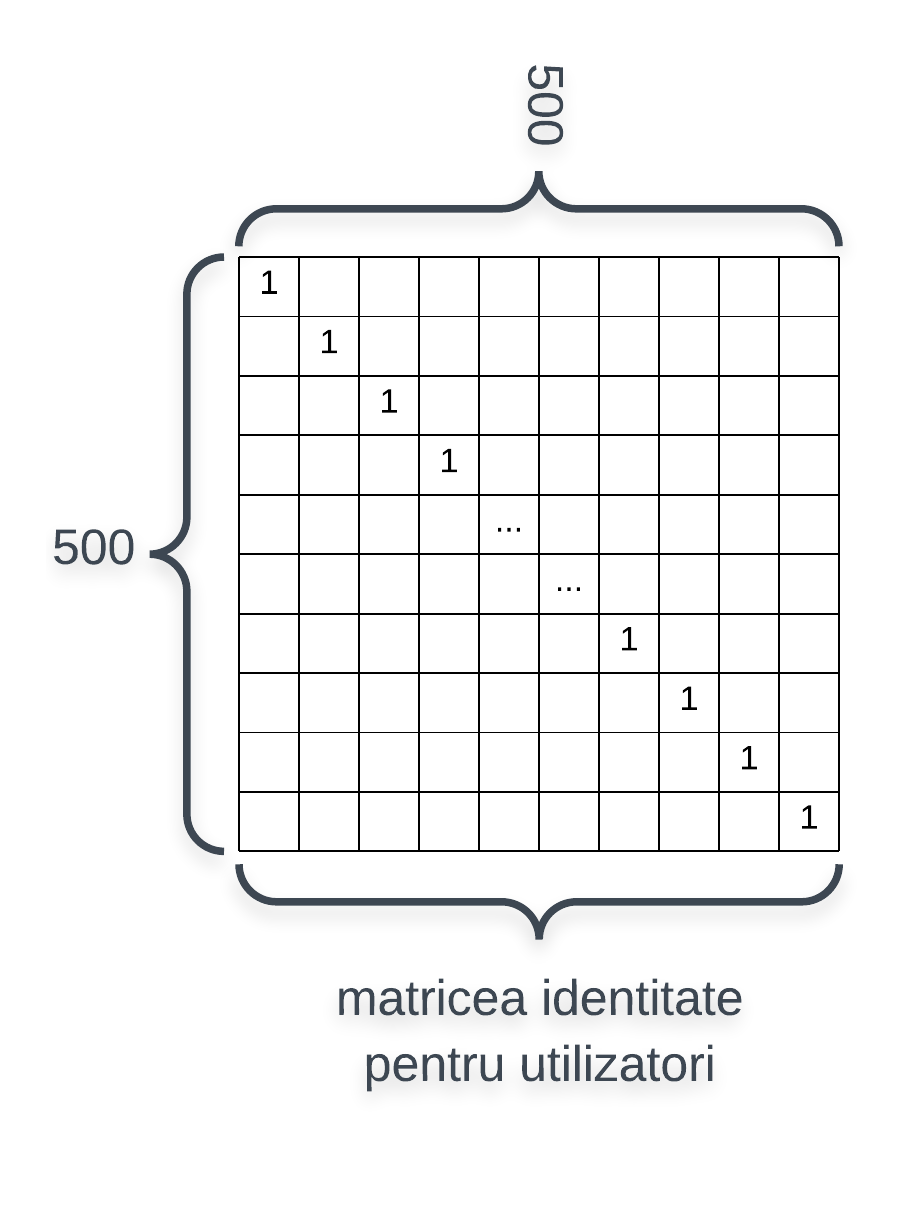
\includegraphics[max width=10cm,max height=10cm,keepaspectratio]{img_3_1}
	\caption[Structura setului de date pentru utilizatori]{Structura setului de date pentru utilizatori.}
\end{figure} 

\begin{figure}[!h]
	\centering
	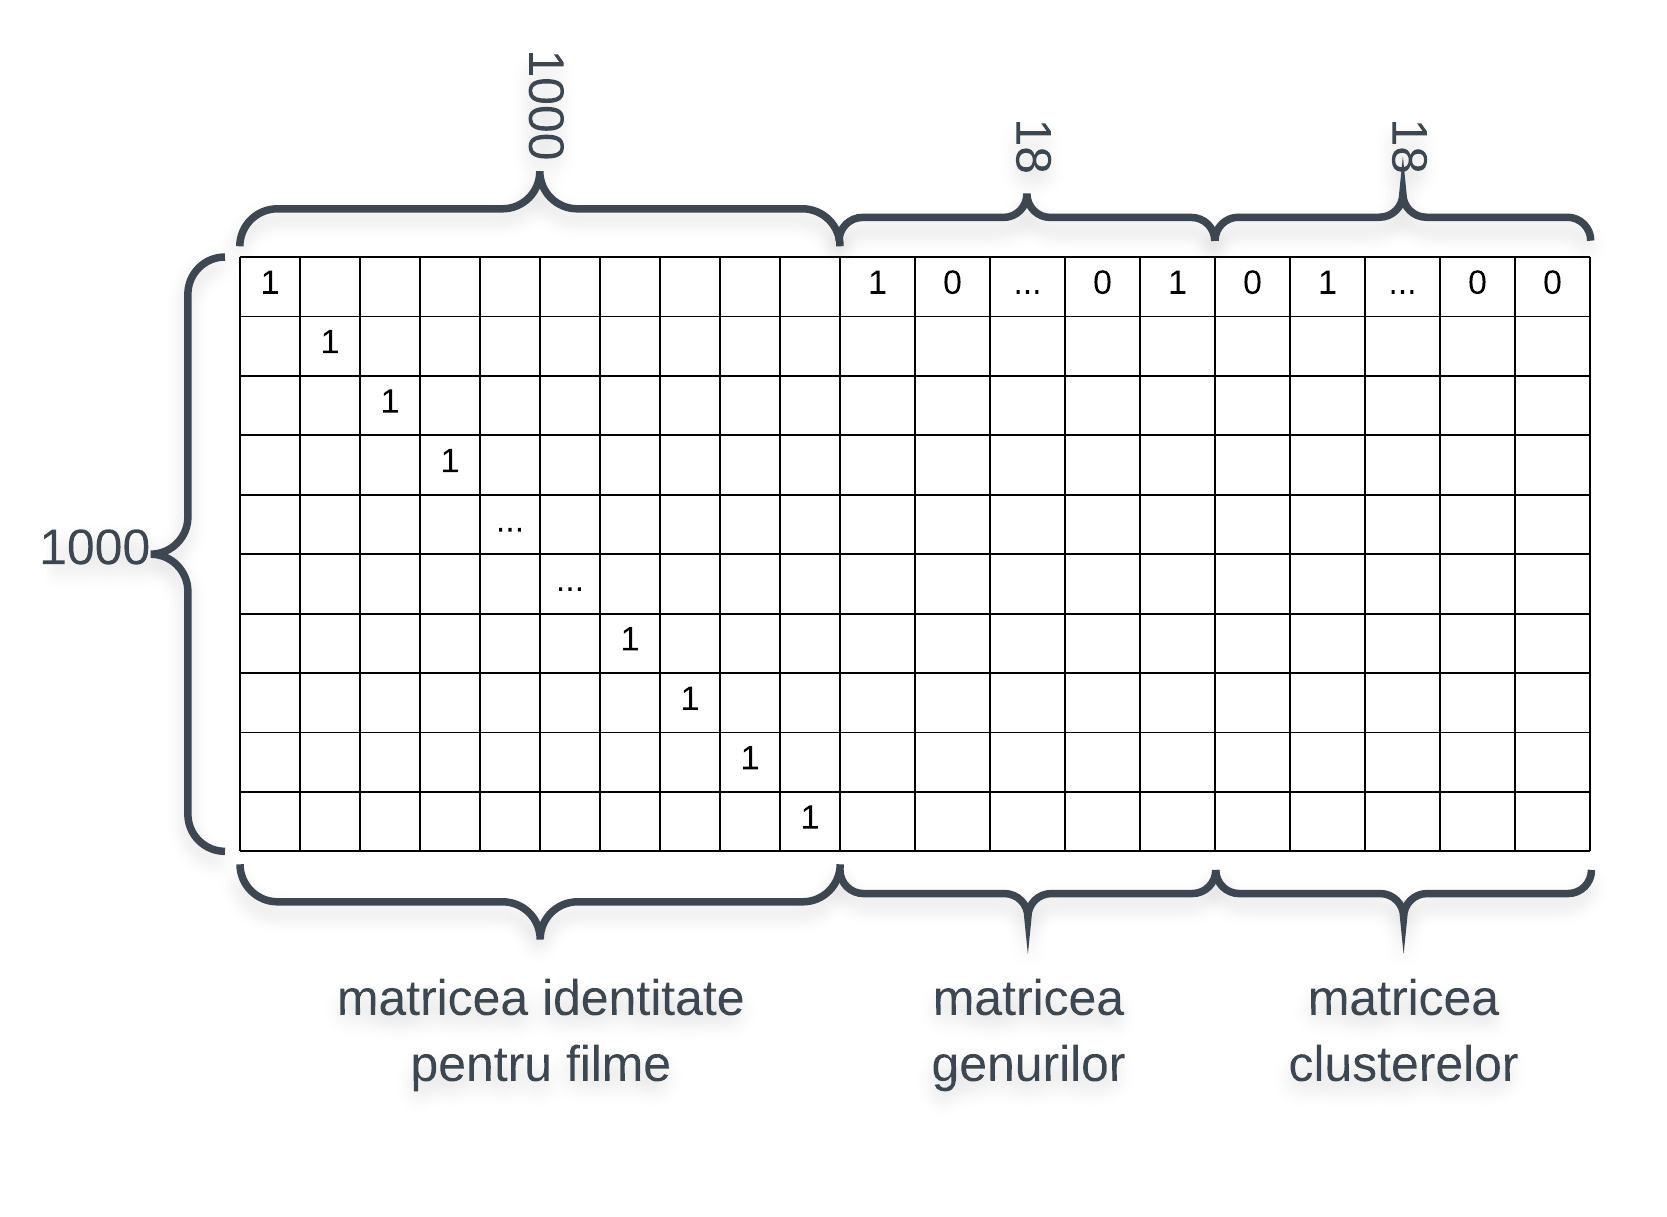
\includegraphics[max width=12cm,max height=12cm,keepaspectratio]{img_3_2}
	\caption[Structura setului de date pentru filme]{Structura setului de date pentru filme.}
\end{figure} 

\section{Optimizarea parametrilor modelului}
De multe ori în algoritmii de machine learning parametrii aleși precum rata de învățare sau numărul de epoci pot influența semnificativ rezultatul final. Astfel, pentru a reduce acest deficit există două variante: prima dintre ele presupune alegerea manuală a acestor parametrii prin diverse încercări; o a doua metodă presupune folosirea unor scripturi/librării specializate în minimizarea unor funcții definite fapt ce automatizează procesul de găsire a parametrilor optimi.

O astfel de librărie este folosită în prezenta lucrare de disertație și anume librăria skopt \hyperlink{skopt}{[22]}. Skopt este o librărie simplă și eficientă care minimizează funcții. Aceasta primește ca input o funcție de minimizat și un spațiu. Spațiul este definit ca fiind mulțimea parametrilor de optimizat și intervalele în care aceștia iau valori, spre exemplu:
\begin{lstlisting}[language=Python, caption=Spațiul parametrilor de optimizat]
space = [(1, 250),  # epochs
        (10 ** -4, 1.0, 'log-uniform'),  # learning_rate
        (20, 200),  # no_components
        (10 ** -6, 10 ** -1, 'log-uniform'),  # item_alpha
        (0.001, 1., 'log-uniform'),  # user_scaling
        (1, 5),  # k for k-OS training
        ] 
\end{lstlisting}

Un exemplu de funcție obiectiv de optimizare este următorea:
\begin{lstlisting}[language=Python, caption=Funcția obiectiv]
def objective(params):
    epochs, learning_rate, no_components, item_alpha, scale = params  # 'k_os'

    user_alpha = item_alpha * scale

    model = LightFM(loss=loss, random_state=2019, learning_rate=learning_rate,
                    no_components=no_components, user_alpha=user_alpha, item_alpha=item_alpha)
    model.fit(train, item_features=item_features, epochs=epochs, num_threads=threads, verbose=True)

    patks = function_to_optimize(model, test, item_features=item_features, num_threads=threads)
    mapatk = np.mean(patks)

    # Make negative because we want to minimize objective
    out = -mapatk

    # Handle some weird numerical shit going on
    if np.abs(out + 1) < 0.01 or out < -1.0:
        return 0.0
    else:
        return out
\end{lstlisting}
unde function\_to\_optimize poate fi una dintre funcțiile de precizie@k sau de acuratețe. De menționat că în cazul acestor două funcții o valoare mai bună înseamnă o valoare mai mare vom face outputul funcției obiectiv negativ astfel încât minimizând funcția obiectiv de fapt să aveam o valoare mai bună pentru funcția de precizie și acuratețe.

Scriptul a fost rulat pentru a optimiza parametrii modelului în următoarele situații:
\begin{enumerate}
	\item \textbf{fără metadate}
	\item \textbf{cu genuri}
	\item \textbf{cu clustere pe rețeaua vgg19, 18 clustere}
	\item \textbf{cu genuri și clustere pe rețeaua vgg19, 18 clustere}
	\item \textbf{cu clustere pe toate celelalte rețele preantrenate, 18 clustere}
	\item \textbf{cu genuri și clustere pe toate celelalte rețele preantrenate, 18 clustere}
\end{enumerate}
Rezultatele obținute se pot vedea în tabelele 3.1 și 3.2. Analizând cele două tabele putem trage următoarele concluzii, pe baza tabelului 3.1:
\begin{enumerate}
	\item funcția de eroare $warp$ obține cele mai bune rezultate atât pe precizie@k cât și pe acuratețe fie că alegem să folosim metadatele în orice combinație a lor, fie că alegem să nu le folosim, fapt pentru care în experimentele efectuate și relatate în tabelul 3.2 am ales să folosim doar această funcție de eroare;
	\item introducerea de metadate este clar o îmbunătățire față de varianta fără aceste metadate;
	\item există o corelație între genuri și clustere pe postere, rezultatele pe acuratețe și precizie fiind destul de apropiate;
	\item modelul de recomandare cu metadatele de clustere converge mai repede către un rezultat optim decât cu metadatele de genuri, atât pe precizie cât și pe acuratețe;
	\item folosite împreună, genurile și clusterele, se obține o îmbunătățire a sistemului de recomandare de aproximativ $1\%$ atât pe acuratețe cât și pe precizie față de modelul fără aceste metadate.
\end{enumerate}

Analizând tabelul 3.2 observăm următoarele:
\begin{enumerate}
	\item cea mai bună precizie și acuratețe pentru un model care folosește doar clustere a fost obținută cu clusterele create prin rețeaua resnet50;
	\item cea mai bună precizie atunci când se folosesc atât genurile cât și clusterele a fost obținută cu clusterele create prin rețeaua vgg19;
	\item cea mai bună acuratețe atunci când se folosesc atât genurile cât și clusterele a fost obținută cu clusterele create prin rețeaua inception\_v3.
\end{enumerate}

\begin{table}
\centering
\caption{Parametrii optimizați pentru modelul de recomandare pe tipuri de feature-uri}
\label{table:1}
\resizebox{\textwidth}{!}{\begin{tabular}{|c|c|c|c|c|c|c|c|c|c|} 
\hline
\multirow{2}{*}{\textbf{Features}} & \multirow{2}{*}{\textbf{Loss}} & \multirow{2}{*}{\textbf{Optimize}} & \multicolumn{6}{c|}{\textbf{Optimal params}}                                                                    & \multirow{2}{*}{\textbf{Results}}  \\ 
\cline{4-9}
                          &                       &                           & \textbf{epochs} & \textbf{learning rate}         & \textbf{no components} & \textbf{item alpha}             & \textbf{scaling}               & \textbf{k os} &                           \\ 
\hline
None                      & warp                  & precision\_at\_k          & 141    & 0.0430  & 21            & 0.0054    & 0.0147  &      & \textbf{0.0920}                    \\ 
\hline
None                      & warp                  & auc\_score                & 93     & 0.0131  & 169           & 2.6154143367150727e-06 & 0.0438   &      & \textbf{0.9309}                    \\ 
\hline
None                      & warp-kos~             & precision\_at\_k          & 131    & 0.0161  & 131           & 0.0148   & 0.0641     & 3    & 0.0915                    \\ 
\hline
None                      & warp-kos~             & auc\_score                & 136    & 0.0253  & 136           & 0.0253   & 0.0014 & 5    & 0.9123                    \\ 
\hline
None                      & bpr                   & precision\_at\_k          & 145    & 0.0118  & 145           & 0.0118   & 0.0087  &      & 0.0818                    \\ 
\hline
None                      & bpr                   & auc\_score                & 100    & 0.3833   & 22            & 0.3833    & 0.6705    &      & 0.8738                    \\ 
\hline
genres                    & warp                  & precision\_at\_k          & 136    & 0.0754     & 82            & 0.0070   & 0.0079   &      & \textbf{0.0990}                    \\ 
\hline
genres                    & warp                  & auc\_score                & 133    & 0.0262  & 193           & 0.0027  & 0.0732  &      & \textbf{0.9384}                    \\ 
\hline
genres                    & warp-kos              & precision\_at\_k          & 106    & 0.0458   & 200           & 0.0058   & 0.0973   & 5    & 0.0968                    \\ 
\hline
genres                    & warp-kos              & auc\_score                & 128    & 0.0313  & 103           & 5.6689548595143295e-06 & 0.2992    & 5    & 0.9184                    \\ 
\hline
genres                    & bpr                   & precision\_at\_k          & 4      & 0.3988    & 174           & 0.0002 & 0.9668    &      & 0.0793                    \\ 
\hline
genres                    & bpr                   & auc\_score                & 113    & 0.3787    & 20            & 1.412418076659026e-06  & 0.8846    &      & 0.8697                    \\ 
\hline
posters                  & warp                  & precision\_at\_k          & 63     & 0.0564   & 98            & 0.0031  & 0.0933    &      & \textbf{0.0938}                    \\ 
\hline
posters                  & warp                  & auc\_score                & 42     & 0.0570    & 68            & 0.0029  & 0.0256   &      & \textbf{0.9338}                    \\ 
\hline
posters                  & warp-kos              & precision\_at\_k          & 111    & 0.1214   & 30            & 0.0051   & 0.2238   & 3    & 0.0900                    \\ 
\hline
posters                  & warp-kos              & auc\_score                & 106    & 0.0206   & 153           & 0.0002  & 0.0172   & 5    & 0.9139                    \\ 
\hline
posters                  & bpr                   & precision\_at\_k          & 112    & 0.0278   & 53            & 0.0430   & 0.0450  &      & 0.0794                    \\ 
\hline
posters                  & bpr                   & auc\_score                & 76     & 0.3969   & 20            & 3.559358324483847e-05  & 0.7491     &      & 0.8656                    \\ 
\hline
genres, posters          & warp                  & precision\_at\_k          & 96     & 0.1703    & 22            & 0.0042   & 0.0413  &      & \textbf{0.0980}                    \\ 
\hline
genres, posters          & warp                  & auc\_score                & 120    & 0.0277  & 189           & 0.0011  & 0.4922    &      & \textbf{0.9406}                    \\ 
\hline
genres, posters          & warp-kos              & precision\_at\_k          & 83     & 0.0748   & 190           & 0.0079   & 0.0124  & 5    & 0.0916                    \\ 
\hline
genres, posters          & warp-kos              & auc\_score                & 149    & 0.0374    & 98            & 6.392983080540728e-05  & 0.6204    & 5    & 0.9205                    \\ 
\hline
genres, posters          & bpr                   & precision\_at\_k          & 19     & 0.0012 & 140           & 9.939007330655304e-05  & 0.0011 &      & 0.0597                    \\ 
\hline
genres, posters          & bpr                   & auc\_score                & 98     & 0.3429    & 21            & 8.687526249607698e-06  & 0.7296    &      & 0.8681                    \\
\hline
\end{tabular}}
\end{table}

\begin{table}
\centering
\caption{Parametrii optimizați pentru modelul de recomandare pe tipuri de feature-uri și modele de rețele preantrenate}
\label{table:2}
\resizebox{\textwidth}{!}{\begin{tabular}{|c|c|c|c|c|c|c|c|c|c|} 
\hline
\multirow{2}{*}{\textbf{Features} } & \multirow{2}{*}{\textbf{Loss }} & \multirow{2}{*}{\textbf{Optimize} } & \multicolumn{5}{c|}{\textbf{Optimal params}}                                                                      & \multirow{2}{*}{\textbf{Model} } & \multirow{2}{*}{\textbf{Results }}  \\ 
\cline{4-8}
                                    &                                 &                                     & \textbf{epochs} & \textbf{learning rate} & \textbf{no components} & \textbf{item alpha}   & \textbf{scaling}      &                                  &                                     \\ 
\hline
posters                            & warp                            & precision\_at\_k                    & 232             & 0.0717    & 42                     & 0.0065  & 0.0161  & vgg19                            & 0.0935                              \\ 
\hline
posters                            & warp                            & auc\_score                          & 89              & 0.0188   & 139                    & 0.0008 & 0.2864    & vgg19                            & 0.9325                              \\ 
\hline
genres, posters                    & warp                            & precision\_at\_k                    & 218             & 0.1247    & 73                     & 0.0054  & 0.0463   & vgg19                            & \textbf{0.0995}                              \\ 
\hline
genres, posters                    & warp                            & auc\_score                          & 236             & 0.0318   & 139                    & 0.0010 & 0.8362    & vgg19                            & 0.9413                              \\ 
\hline
posters                            & warp                            & precision\_at\_k                    & 119             & 0.0085    & 192                    & 7.276515301192984e-05 & 0.0270  & inception\_v3                    & 0.0836                              \\ 
\hline
posters                            & warp                            & auc\_score                          & 232             & 0.0298    & 84                     & 0.0042  & 0.0405  & inception\_v3                    & 0.9327                              \\ 
\hline
genres, posters                    & warp                            & precision\_at\_k                    & 245             & 0.0289   & 43                     & 0.0006 & 0.3657   & inception\_v3                    & 0.0905                              \\ 
\hline
genres, posters                    & warp                            & auc\_score                          & 250             & 0.0194   & 136                    & 0.0008 & 0.4767    & inception\_v3                    & \textbf{0.9425}                              \\ 
\hline
posters                            & warp                            & precision\_at\_k                    & 88              & 0.0749    & 21                     & 0.0046  & 0.0281  & resnet50                         & \textbf{0.0953}                              \\ 
\hline
posters                            & warp                            & auc\_score                          & 198             & 0.0167   & 169                    & 0.0012 & 0.6692    & resnet50                         & \textbf{0.9342}                              \\ 
\hline
genres, posters                    & warp                            & precision\_at\_k                    & 224             & 0.0421    & 186                    & 0.0086  & 0.0024 & resnet50                         & 0.0970                              \\ 
\hline
genres, posters                    & warp                            & auc\_score                          & 211             & 0.0976    & 48                     & 0.0034  & 0.1123   & resnet50                         & 0.9397                              \\
\hline
\end{tabular}}
\end{table}

În capitolul următor sunt utilizați acești parametrii optimi găsiți pentru a studia evoluția performanței modelului în timp, studiu ce ne va permite să tragem concluziile finale.

\newpage\null\newpage
\chapter{Evaluarea experimentală}
\section{Bază de date filme}
În cadrul prezentei diserații a fost folosită ca bază de date pentru evaluarea experimentală baza oferita de grouplens \hyperlink{movielens}{[22]}. Aceștia pun la dispoziție mai multe seturi de date printre care:
\begin{enumerate}
	\item \textbf{MovieLens 20M Dataset}: conține 20 milioane de ratinguri oferite de 138 000 de utilizatori peste 27 000 de filme;
	\item \textbf{MovieLens 10M Dataset}: conține 10 milioane de ratinguri oferite de 72 000 de utilizatori peste 10 000 de filme;
	\item \textbf{MovieLens 1M Dataset}: conține 1 milion de ratinguri oferite de 6 000 de utilizatori peste 4 000 de filme.
\end{enumerate}

În evaluarea curentă a fost folosită cea mai recentă versiune de bază de date, actualizată la 9/2018, de dimensiune mică și anume \textit{ml-latest-small}. Această bază de date conține 100 000 de ratinguri și 3 600 de taguri aplicate peste 9 000 de filme de 600 de utilizatori. Această bază de date este un subset dintr-o bază de date cu 27 de milioane de ratinguri și 1 milion de taguri, aplicate peste 58 000 de filme de 280 000 de utilizatori.

Fiecare utilizator din \textit{ml-latest-small} a acordat ratinguri pentru cel puțin 20 de filme. Baza de date nu conține informații demografice, fiecare utilizator fiind reprezentat doar de un id.

Structura fișierelor din baza de date:
\begin{itemize}
	\item \textbf{ratings.csv}: fiecare linie din acest fișier reprezintă un rating dat de un utilizator unui film, fișierul având formatul $userId, movieId, rating, timestamp$, unde $timestamp$ reprezintă momentul de timp când a fost acordat ratingul. Fiecare rating este cuprins între 0 și 5, iar între ratinguri este unpas de 0.5;
	\item \textbf{movies.csv}: conține metadate despre filme precum titlul și genul. Formatul fișierului este următorul: $movieId, title, genres$. Titlul conține și anul de apariție a filmului sub forma \textit{Titlu (an)}. Genul poate fi unul sau mai multe dintre următoarele: \textit{Action, Adventure, Animation, Children's, Comedy, Crime, Documentary, Drama, Fantasy, Film-Noir, Horror, Musical, Mystery Romance, Sci-Fi, Thriller, War Western, (no genres listed)}.
	\item \textbf{links.csv}: conține referințele către site-urile movielens, imdb și themoviedb sub următorul format: $movieId,imdbId,tmdbId$.
	\item \textbf{tags.csv}: fiecare linie conține un tag aplicat de un utilizator unui film, fișierul având următorul format $userId,movieId,tag,timestamp$. Fiecare tag este reprezentat de un cuvânt sau de o scurtă frază.
\end{itemize}

\section{Bază de date postere}
În ceea ce privește baza de date pentru postere, aceasta a fost construită în cadrul dezvoltării prezentei lucrări cu ajutorul a două elemente: fișierul de \textit{links} din setul de date \textit{ml-latest-small} și cu API-ul pus la dispoziție de către platforma \textbf{themoviedb.org} \hyperlink{themoviedb}{[24]}.

Procesul de construcție a acestui set de postere pentru filme poate fi rezumat pe pași după cum urmează:
\begin{enumerate}
	\item \textbf{Pasul 1}: extragerea id-urilor filmelor aferente platformei themoviedb.org;
	\item \textbf{Pasul 2}: pentru fiecare film se face un request către API pentru a lua lista de postere pentru filmul curent;
	\item \textbf{Pasul 3}: având adresele posterelor pentru filmul curent, se descarcă și se salvează posterele la dimensiunea originală într-un folder specific filmului.
\end{enumerate}
Din punct de vedere al implementării putem menționa funcțiile:
\begin{lstlisting}[language=Python, caption=Construcția setul de date cu postere]
def get_tmdb_posters(tmdb_api_key, max_movie_posters=10):
    # pasul 1    
    tmdb_movies_id = get_tmdb_ids()
    # pasul 2 - 3
    download_images(tmdb_api_key, tmdb_movies_id, max_movie_posters)

# unde download_images are urmatoarea definitie:
def download_images(tmdb_api_key, tmdb_movies_id, max_movie_posters=10):
\end{lstlisting}
unde:
\begin{itemize}
	\item \textbf{tmdb\_api\_key} este api key-ul unic asociat unui cont pe platforma themoviedb.org care a solicitat acces la API-ul platformei;
	\item \textbf{max\_movie\_posters} definește care este numărul maxim de postere care va fi descărcat pentru un film. Numărul de postere descărcate poate fi mai mic în cazul în care nu sunt cel puțin max\_movie\_posters.
\end{itemize}

\begin{figure}[!tbp]
  \begin{subfigure}[b]{0.3\textwidth}
    
\includegraphics[width=9cm,height=5cm,keepaspectratio]{img_4_1}
  \end{subfigure}
  \hfill
  \begin{subfigure}[b]{0.3\textwidth}
    
\includegraphics[width=9cm,height=5cm,keepaspectratio]{img_4_2}
  \end{subfigure}
  \hfill
  \begin{subfigure}[b]{0.3\textwidth}
    
\includegraphics[width=9cm,height=5cm,keepaspectratio]{img_4_3}
  \end{subfigure}
  \hfill
  \begin{subfigure}[b]{0.3\textwidth}
    
\includegraphics[width=9cm,height=5cm,keepaspectratio]{img_4_4}
  \end{subfigure}
  \hfill
  \begin{subfigure}[b]{0.3\textwidth}
    
\includegraphics[width=9cm,height=5cm,keepaspectratio]{img_4_5}
  \end{subfigure}
  \hfill
  \begin{subfigure}[b]{0.3\textwidth}
    
\includegraphics[width=9cm,height=5cm,keepaspectratio]{img_4_6}
  \end{subfigure}
  \caption[Exemple de postere]{Exemplu de postere pentru filmul Paddington 2.}
\end{figure}

\section{Rezultate clusterizare postere}

\subsection{Sanity check}
Pentru testarea validității clasterelor un test de sanity check în care s-au luat opt filme și s-a încercat clasificarea lor în șapte clastere folosind caracteristicile extrase din rețelele preantrenate VGG16, VGG19, InceptionV3, ResNet50 și NASNet, clasterele create cu kNN iar evaluarea este făcută atât vizual cât și prin urmărirea evoluției metricii silhouette de la 2 la 7 clastere. Posterele de input pentru sanity check sunt prezentate în figura 4.2.
\begin{figure}[!tbp]
  \centering
  \begin{subfigure}[b]{0.48\textwidth}
    \includegraphics[width=\textwidth]{img_4_7}
  \end{subfigure}
  \hfill
  \begin{subfigure}[b]{0.48\textwidth}
    \includegraphics[width=\textwidth]{img_4_8}
  \end{subfigure}
    \hfill
  \begin{subfigure}[b]{0.48\textwidth}
    \includegraphics[width=\textwidth]{img_4_9}
  \end{subfigure}
  \hfill
  \begin{subfigure}[b]{0.48\textwidth}
    \includegraphics[width=\textwidth]{img_4_10}
  \end{subfigure}
  \hfill
  \begin{subfigure}[b]{0.48\textwidth}
    
\includegraphics[width=\textwidth]{img_4_11}
  \end{subfigure}
  \hfill
  \begin{subfigure}[b]{0.48\textwidth}
    
\includegraphics[width=\textwidth]{img_4_12}
  \end{subfigure}
    \hfill
  \begin{subfigure}[b]{0.48\textwidth}
    
\includegraphics[width=\textwidth]{img_4_13}
  \end{subfigure}
    \hfill
  \begin{subfigure}[b]{0.48\textwidth}
    
\includegraphics[width=\textwidth]{img_4_14}
  \end{subfigure}
      \hfill
  \begin{subfigure}[b]{0.3\textwidth}
    
\includegraphics[width=\textwidth]{img_4_15}
  \end{subfigure}
  \caption[Postere input sanity check]{Posterele de input pentru sanity check.}
\end{figure}

Din punct de vedere al metricii de evaluare silhouette rezultatele se prezintă după cum urmează în figura 4.3.
\begin{figure}[!h]
	\centering
	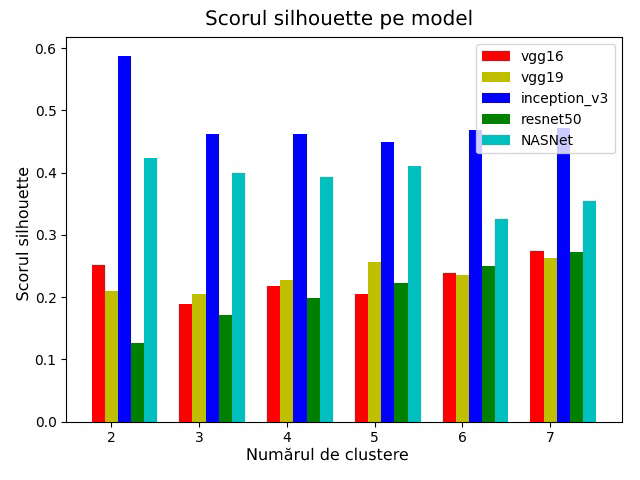
\includegraphics[max width=12cm,max height=12cm,keepaspectratio]{img_4_16}
	\caption[Silhouette score pentru clasterele din sanity check]{Silhouette score pentru clasterele din sanity check.}
\end{figure} 

\subsection{Rezultate generale}

\section{Rezultate sistem de recomandare}


\newpage\null\newpage
\chapter*{Concluzii}
\addcontentsline{toc}{chapter}{Concluzii} 
Concluziile disertației ...

\begin{thebibliography}{9}

	\bibitem{domo}
	\hypertarget{domo}{} 
	Data never sleeps 6.0
	\\\texttt{\url{https://www.domo.com/learn/data-never-sleeps-6}}
	
	\bibitem{finder}
	\hypertarget{finder}{} 
	Netflix International: What movies and TV shows can I watch, and where can I watch them?
	\\\texttt{\url{https://www.finder.com/global-netflix-library-totals}}

	\bibitem{scrapehero}
	\hypertarget{scrapehero}{} 
	How Many Products Does Amazon Sell? – April 2019
	\\\texttt{\url{https://www.scrapehero.com/number-of-products-on-amazon-april-2019/}}
	
	\bibitem{ErionCanoMaurizioMorisio}
	\hypertarget{ErionCanoMaurizioMorisio}{} 
	Erion Çano, Maurizio Morisio.
	\textit{\href{https://arxiv.org/abs/1901.03888}{Hybrid Recommender Systems: A Systematic Literature Review}}.
	Intelligent Data Analysis, vol. 21, no. 6, pp. 1487-1524, 2017
	
	\bibitem{datameetsmedia}
	\hypertarget{datameetsmedia}{} 
	An Overview of Recommendation Systems
	\\\texttt{\url{http://datameetsmedia.com/an-overview-of-recommendation-systems/}}
	
	\bibitem{lightfm}
	\hypertarget{lightfm}{} 
	LightFM 1.15 - documentation
	\\\texttt{\url{http://lyst.github.io/lightfm/docs/lightfm.html}}
	
	\bibitem{cs231n}
	\hypertarget{cs231n}{} 
	CS231n: Convolutional Neural Networks for Visual Recognition
	\\\texttt{\url{http://cs231n.stanford.edu/2018/syllabus.html}}
	
	\bibitem{JasonWestonSamyBengioNicolasUsunier}
	\hypertarget{JasonWestonSamyBengioNicolasUsunier}{} 
	Jason Weston, Samy Bengio, Nicolas Usunier.
	\textit{\href{http://www.thespermwhale.com/jaseweston/papers/wsabie-ijcai.pdf}{Wsabie: Scaling up to large vocabulary image annotation}}.
	IJCAI. Vol. 11. 2011.
	
	\bibitem{SteffenRendleChristophFreudenthalerZenoGantnerLarsSchmidtThieme}
	\hypertarget{SteffenRendleChristophFreudenthalerZenoGantnerLarsSchmidtThieme}{} 
	Steffen Rendle, Christoph Freudenthaler, Zeno Gantner and Lars Schmidt-Thieme.
	\textit{\href{http://www.thespermwhale.com/jaseweston/papers/wsabie-ijcai.pdf}{BPR: Bayesian personalized ranking from implicit feedback}}.
	Proceedings of the Twenty-Fifth Conference on Uncertainty in Artificial Intelligence. AUAI Press, 2009.
	
	\bibitem{SimonyanKarenZissermanAndrew}
	\hypertarget{SimonyanKarenZissermanAndrew}{} 
	Karen Simonyan, Andrew Zisserman.
	\textit{\href{https://arxiv.org/pdf/1409.1556.pdf}{Very Deep Convolutional Networks for Large-Scale Image Recognition}}.
	 ICLR, 2015.
	 
	\bibitem{KaimingHeXiangyuZhangShaoqingRenJianSun}
	\hypertarget{KaimingHeXiangyuZhangShaoqingRenJianSun}{} 
	Kaiming He, Xiangyu Zhang, Shaoqing Ren, Jian Sun.
	\textit{\href{https://arxiv.org/pdf/1512.03385.pdf}{Deep Residual Learning for Image Recognition}}.
	 IEEE Conference on Computer Vision and Pattern Recognition (CVPR), p770-778, 2016.

	\bibitem{Szegedy2016RethinkingTI}
	\hypertarget{Szegedy2016RethinkingTI}{} 
	Christian Szegedy, Vincent Vanhoucke, Sergey Ioffe, Jonathon Shlens, Zbigniew Wojna.
	\textit{\href{https://arxiv.org/pdf/1512.00567.pdf}{Rethinking the Inception Architecture for Computer Vision}}.
	 IEEE Conference on Computer Vision and Pattern Recognition (CVPR), p2818-2826, 2016.	
	
	\bibitem{Zoph2018LearningTA}
	\hypertarget{Zoph2018LearningTA}{} 
	Barret Zoph, Vijay Vasudevan, Jonathon Shlens, Quoc V. Le.
	\textit{\href{https://arxiv.org/pdf/1707.07012.pdf}{Learning Transferable Architectures for Scalable Image Recognition}}.
	 IEEE/CVF Conference on Computer Vision and Pattern Recognition, p8697-8710, 2018.	
	
	\bibitem{guideinceptionv3}
	\hypertarget{guideinceptionv3}{} 
	Advanced Guide to Inception v3 on Cloud TPU
	\\\texttt{\url{https://cloud.google.com/tpu/docs/inception-v3-advanced}}
	
	\bibitem{dataclusteringtechniques}
	\hypertarget{dataclusteringtechniques}{} 
	Data Clustering Techniques
	\\\texttt{\url{http://www.cs.toronto.edu/~periklis/pubs/depth.pdf}}
	
	\bibitem{gongdeguo}
	\hypertarget{gongdeguo}{} 
	Gongde Guo, Hui Wang, David Bell, Yaxin Bi, Kieran Greer.
	\textit{\href{http://citeseerx.ist.psu.edu/viewdoc/download?doi=10.1.1.2.815&rep=rep1&type=pdf}{KNN Model-Based Approach in Classification}}.
	Lecture Notes in Computer Science, vol 2888. Springer, Berlin, Heidelberg, 2003.

	\bibitem{silhouette}
	\hypertarget{silhouette}{} 
	Sklearn metrics - silhouette score
	\\\texttt{\url{https://scikit-learn.org/stable/modules/generated/sklearn.metrics.silhouette_score.html}}
\end{thebibliography}


\end{document}